\documentclass[aspectratio=169,11pt]{beamer}
\usepackage[UTF8,fontset=none]{ctex}
\setCJKmainfont{Microsoft JhengHei}
\setCJKsansfont{Microsoft JhengHei}
\usepackage{amsmath,amssymb,booktabs,array}
\usepackage{pgfplots}
\pgfplotsset{compat=1.18}
\definecolor{navy}{HTML}{183750}
\definecolor{teal}{HTML}{007E87}
\definecolor{orange}{HTML}{B45A20}
\setbeamercolor{normal text}{fg=navy,bg=white}
\setbeamercolor{structure}{fg=teal}
\setbeamercolor{frametitle}{fg=navy}
\setbeamercolor{alerted text}{fg=orange}
\setbeamerfont{frametitle}{size=\Large,series=\bfseries}
\setbeamertemplate{navigation symbols}{}
\setbeamertemplate{itemize items}[circle]
\setbeamersize{text margin left=8mm,text margin right=8mm}
\setbeamertemplate{footline}{\hspace{8mm}\scriptsize 第三章自讀筆記\hfill\insertsectionhead\hfill\insertframenumber/\inserttotalframenumber\hspace{8mm}\vspace{3mm}}
\newcommand{\src}[1]{\par\vfill{\scriptsize\color{teal}教材：#1。頁碼均為書本印刷頁碼。}}
\newcommand{\slide}[3]{\begin{frame}[t]{#1}#3\src{#2}\end{frame}}
\newcommand{\bi}{\begin{itemize}\setlength{\itemsep}{5pt}}
\newcommand{\ei}{\end{itemize}}
\newcommand{\key}[1]{\par\medskip{\color{teal}\bfseries #1}\par\smallskip}
\newcommand{\dd}{\mathrm{d}}
\title{空氣動力學與飛機控制}
\subtitle{Introduction to Avionics Systems 第三章\\完整自讀詳解}
\author{依 R. P. G. Collinson，第 3 版整理}
\date{教材 pp. 101--177}

% Original images extracted losslessly from the supplied textbook PDF.
\newcommand{\originalfigure}[6]{
\begin{frame}[t]{課本原圖 #1：#2}
\centering
\includegraphics[width=.94\linewidth,height=5.05cm,keepaspectratio]{figures/#4}\par
\vspace{2mm}\raggedright\small #5\par
\vfill{\scriptsize\color{teal}原圖：Collinson, 第 3 版，Fig. #1，p. #3。#6}\par
\end{frame}}

\begin{document}
\begin{frame}\titlepage\centering\small 概念、模型、推導、算例與自我檢查\end{frame}

\section{閱讀地圖}
\slide{這一章要建立的能力}{3.1，p. 101}{
\bi
\item 從升力、阻力與力矩，理解飛機為何能配平，以及受擾動後是否會恢復。
\item 從機體座標與 Newton 定律，建立小擾動運動方程。
\item 用氣動導數、狀態空間與傳遞函數，描述操縱面輸入造成的動態響應。
\item 理解 PCU、穩定增強系統（SAS）與直升機控制，如何連接到後續的 FBW。
\ei
\key{閱讀主線}力與力矩的來源，決定運動模型。模型的模態與限制，決定控制系統需要改善什麼。
}
\slide{分次閱讀安排}{3.1--3.9，pp. 101--177}{
\small
\begin{tabular}{p{.15\textwidth}p{.49\textwidth}p{.22\textwidth}}
\toprule 單元 & 核心問題 & 教材範圍\\\midrule
基礎氣動 & 升力、阻力與配平力矩如何產生？ & 3.2，101--110\\
穩定性 & 受擾動後，初始趨勢與時間響應如何？ & 3.3，110--114\\
動力學 & 如何把力學寫成可計算的線性模型？ & 3.4，115--134\\
縱向控制 & 升降舵如何改變迎角與俯仰角速度？ & 3.5，134--148\\
橫向控制 & 副翼、方向舵如何形成轉彎與耦合？ & 3.6，148--153\\
致動與增穩 & 液壓伺服、回授與冗餘的作用？ & 3.7--3.8，154--162\\
直升機 & 旋翼操控與四個控制軸如何互相影響？ & 3.9，163--177\\\bottomrule
\end{tabular}
}
\slide{範圍與閱讀約定}{全章；原始檔 textbook.pdf}{
\bi
\item 來源：R. P. G. Collinson, \textit{Introduction to Avionics Systems}, 3rd ed., Springer, 2011，第 3 章。
\item 對應 PDF 檔案第 116--192 頁，共 77 個實際頁面，包含章末 Further Reading。
\item 「補充推導」是依教材模型延伸的計算。「核對提醒」說明算術、正負號或模型階數的問題。
\item 機型、典型數值與可靠度範例屬出版時敘述，不當作現行規範或所有機型的通則。
\ei
\key{使用方式}先讀物理意義，再核對假設與符號，最後自行推導公式和算例。
}

\section{3.2 基礎空氣動力學}
\slide{升力與阻力的兩種描述}{3.2.1，pp. 101--103}{
\bi
\item 壓力觀點：翼面各處壓力分布與表面剪應力，積分後形成合力。教材以翼上減壓、翼下增壓作直觀說明。
\item 動量觀點：機翼使流過的空氣改變動量，空氣對機翼施加反作用力。
\item 兩種觀點描述同一個氣動作用，不能把它們當成兩份可相加的升力來源。
\item 升力垂直於相對氣流，阻力沿相對氣流方向，與飛機相對空氣的運動方向相反。
\ei
\key{閱讀提醒}教材的「上表面約占三分之二」是示意比例，不能套用到所有翼型、迎角與飛行條件。
}
\originalfigure{3.1}{翼面壓力分布}{102}{fig-3-01.png}{比較上、下翼面的壓力分布，並將分布力連到合升力。}{}

\originalfigure{3.2}{氣流動量與反作用力}{102}{fig-3-02.png}{觀察氣流偏轉與動量改變，這與壓力分布是同一氣動作用的兩種描述。}{}

\slide{迎角、姿態與航跡角}{3.2.2，p. 103；角度關係為補充}{
\bi
\item 迎角（angle of attack），$\alpha$：翼弦基準線與相對氣流方向的夾角。
\item 教材用 angle of incidence 表示迎角。其他資料中的 incidence 也可能指機翼安裝角。
\item 俯仰角 $\theta$ 表示機體姿態，航跡角 $\gamma$ 表示速度向量相對水平面的方向。
\ei
\[\alpha\simeq\theta-\gamma\]
此式假設縱向平面運動，且翼弦與機體基準線一致。若有固定安裝角，必須另行計入。
\key{例子}抬頭姿態不保證正在爬升。飛機可能在很大的迎角下仍然下降。
}
\originalfigure{3.3}{迎角、升力與阻力方向}{103}{fig-3-03.png}{迎角以翼弦與相對氣流為基準，升力方向未必等於機體向上方向。}{}

\slide{動壓與氣動係數}{3.2.3，p. 104，式 (3.1)--(3.5)}{
\[Q=\frac12\rho V_T^2,\qquad L_W=QS C_L,\qquad D_W=QS C_D\]
\bi
\item $\rho$：空氣密度，$\mathrm{kg/m^3}$。$V_T$：相對空氣的速度，$\mathrm{m/s}$。
\item $Q$：動壓，單位 $\mathrm{Pa=N/m^2}$。$S$：機翼參考面積，$\mathrm{m^2}$。
\item $C_L,C_D$ 無因次，包含翼型、迎角與流況等影響。力的大小由動壓、面積與係數共同決定。
\item 保留大寫 $Q$ 表示動壓，避免與俯仰角速度 $q$ 混淆。
\ei
\key{適用限制}可壓縮流的衝壓差不直接等於 $\frac12\rho V_T^2$，但動壓仍可用此式定義。
}
\slide{升力曲線與失速}{3.2.3，pp. 104--105}{
\[C_L\simeq C_{L0}+C_{L\alpha}\alpha
       =C_{L\alpha}(\alpha-\alpha_{L=0})\]
\bi
\item 失速前的一段迎角範圍可近似線性。斜率 $C_{L\alpha}$ 必須註明每度或每弧度。
\item 超過臨界迎角後，分離流使升力曲線不再遵守線性式，不能繼續外插。
\item 教材典型值：一般翼型 $C_{L\max}\approx1.2$--$1.6$，臨界迎角約 $15^\circ$--$20^\circ$，三角翼可更高。
\item 失速與迎角有關。所謂失速速度，還依重量、密度、載荷因數與構型而變。
\ei
}
\originalfigure{3.4}{升阻力係數與迎角}{105}{fig-3-04.png}{注意失速附近的升力曲線轉折，以及大迎角下阻力的增加。}{}

\slide{阻力極線與高升力裝置}{3.2.3，pp. 104--106，式 (3.6)}{
\[C_D\simeq C_{D0}+kC_L^2\]
\bi
\item $C_{D0}$ 表示此模型中與升力平方項分離的基礎阻力，$kC_L^2$ 描述隨升力增加的阻力。
\item 需要更大的 $C_L$ 時，阻力通常增加，維持速度就需要更多推力。
\item 前緣縫翼、前緣襟翼與後緣襟翼改變翼型／流動，增加可用升力。教材列舉高升力構型 $C_{L\max}$ 可達約 3--4。
\item 接近音速時，壓縮性會明顯改變 $C_L,C_D$。不可用同一組低速係數涵蓋整個飛行包線。
\ei
}
\originalfigure{3.5}{前緣縫翼與後緣襟翼}{106}{fig-3-05.png}{比較高升力裝置伸出與收回時，升力係數對迎角的變化。}{}

\slide{等速平飛與低速限制}{3.2.3--3.2.4，pp. 104--107；補充推導}{
忽略尾翼分擔、推力垂直分量等因素，等速平飛近似有
\[L\simeq mg,\quad T\simeq D,\quad
C_{L,\mathrm{req}}=\frac{2mg}{\rho V_T^2S}.\]
\bi
\item 同一重量與密度下，速度減半，需要的 $C_L$ 增為四倍。
\item 密度降低時，維持相同真空速與升力需要更高的 $C_L$。
\item 可用升力係數存在上限，因此 $V_s=\sqrt{2mg/(\rho S C_{L\max})}$。
\ei
\key{補充}載荷因數為 $n=L/(mg)$ 時，在同一構型與密度下，$V_{s,n}=V_{s,1}\sqrt n$。
}
\slide{教材算例：低空低速的迎角}{3.2.4，pp. 105--107}{
\small
已知 $m=30{,}000\ \mathrm{kg}$，$S=75\ \mathrm{m^2}$，$\rho=1.225\ \mathrm{kg/m^3}$，$V_T=80\ \mathrm{m/s}$。
\[Q=\tfrac12(1.225)(80)^2=3920\ \mathrm{Pa}\]
\[C_L=\frac{30{,}000(9.81)}{3920(75)}=1.001\approx1.0\]
教材特別假設升力曲線通過原點，且 $C_{L\max}=1.2$ 對應 $\alpha_{\max}=15^\circ$。
\[C_{L\alpha}=\frac{1.2}{15}=0.08/\mathrm{deg},\qquad
\alpha\approx\frac{1.0}{0.08}=12.5^\circ\]
\key{意義}這個低速平飛條件已接近教材設定的臨界迎角，進一步增加升力的餘裕有限。
}
\slide{教材算例：速度與可用機動加速度}{3.2.4，pp. 106--107}{
\small
同一低空密度，改為 $200\ \mathrm{m/s}$ 平飛：
\[\alpha\approx12.5^\circ\left(\frac{80}{200}\right)^2=2.0^\circ.\]
高度 $30{,}000\ \mathrm{ft}$，$\rho=0.4583$，$V_T=225\ \mathrm{m/s}$：
\[L_{\max}=\tfrac12(0.4583)(225)^2(75)(1.2)
\approx1.044\times10^6\ \mathrm{N}.\]
\[n_{\max}=\frac{L_{\max}}{mg}\approx3.55,\qquad
\frac{L_{\max}-mg}{m}\approx25.0\ \mathrm{m/s^2}\approx2.55g.\]
\key{兩個不同量}3.55 是升力／重量的載荷因數。2.55$g$ 是此算例扣除重力後的向上淨加速度。教材的「2.5$g$」指後者。
}
\slide{壓力中心與氣動中心}{3.2.5，pp. 107--108}{
\bi
\item 壓力中心（centre of pressure）：合氣動力的作用位置，關於此點的合力矩為零。位置隨迎角改變。
\item 氣動中心（aerodynamic centre, AC）：在所考慮條件下，關於此點的俯仰力矩對迎角變化近似不變。
\item 使用 AC 可把機翼等效為作用於固定位置的氣動力，加上一個近似固定的俯仰偶矩。
\item 教材的近似位置：亞音速約四分之一翼弦，超音速趨近二分之一翼弦。整機 AC 與單獨機翼 AC 必須區分。
\ei
\[M_0=QSc C_{M0},\qquad [QSc]=\mathrm{N\,m}.\]
}
\slide{尾翼如何平衡俯仰力矩}{3.2.6，pp. 108--110，式 (3.9)--(3.12)}{
採教材圖 3.6 的配置，$x>0$ 表示機翼升力作用點在 CG 後方，$L_t>0$ 表示向下的尾翼力大小，$M_0>0$ 表示低頭偶矩大小。
\[M=-L_Wx-M_0+L_tl_t,\qquad L_t=k_tQS_t C_{Lt}\]
\[C_M=-\frac{x}{c}C_L-C_{M0}
       +k_t\frac{S_tl_t}{Sc}C_{Lt}.\]
\bi
\item 尾翼向下作用時，關於 CG 產生抬頭力矩，抵銷其他低頭力矩。
\item $k_t$ 為尾翼處動壓／自由流動壓，教材典型範圍 0.65--0.95。
\item $S_tl_t$ 稱尾翼容積，$S_tl_t/(Sc)$ 為無因次尾翼容積比。
\ei
}
\originalfigure{3.6}{主翼與尾翼的配平作用}{108}{fig-3-06.png}{依 CG、機翼氣動中心與尾翼力臂，逐項核對力矩正負號。}{}

\slide{配平的代價與幾何量提醒}{3.2.5--3.2.6，pp. 108--110}{
\bi
\item 向下尾翼力使總向上升力減少。因此主翼需提供 $L_W=mg+L_t$，而非只提供 $mg$。
\item 尾翼面積或力臂增大，通常可增加控制力矩與恢復作用，但會付出重量、阻力等代價。
\item 配平只要求合力與合力矩滿足指定運動。穩定性要另外檢查受擾後的變化率。
\ei
\key{核對提醒：平均翼弦}教材以 $c=S/b$ 作簡化。一般非矩形機翼的平均氣動弦長（MAC）不必等於 $S/b$。本章算式使用給定的參考弦長 $c$，不把此簡化當作通則。
}
\originalfigure{3.7}{機翼與尾翼力矩的疊加}{110}{fig-3-07.png}{合成曲線的零點決定配平迎角，斜率則反映靜恢復作用。}{}


\section{3.3 飛機穩定性}
\slide{靜穩定與動穩定}{3.3，pp. 110--111}{
\small
\begin{tabular}{p{.18\textwidth}p{.65\textwidth}}
\toprule 類型 & 要觀察的量\\\midrule
靜穩定 & 受擾後，初始力或力矩是否朝恢復平衡的方向？\\
靜中性 & 受擾後沒有一階恢復力／力矩，也沒有一階發散趨勢。\\
靜不穩定 & 初始力或力矩使偏離程度增加。\\
動穩定 & 完整時間響應是否衰減回到平衡？需考慮慣性、阻尼與耦合。\\\bottomrule
\end{tabular}
\key{重要區分}有恢復力矩不代表振盪一定衰減。若阻尼不足或為負，系統仍可能持續振盪或動態發散。
\key{配平與穩定}配平決定平衡點的位置，穩定性決定平衡點附近的行為。
}
\originalfigure{3.8}{穩定、中性與不穩定的類比}{110}{fig-3-08.png}{比較小球離開平衡位置後，受到的作用是否促使它回到原處。}{}

\originalfigure{3.9(a)}{靜穩定的初始趨勢}{111}{fig-3-09a.png}{分別觀察初始恢復趨勢，以及時間響應的振幅是否衰減。}{}

\originalfigure{3.9(b)}{動穩定的振幅變化}{111}{fig-3-09b.png}{分別觀察初始恢復趨勢，以及時間響應的振幅是否衰減。}{}

\slide{縱向靜穩定判據}{3.3.1，pp. 110--112}{
抬頭力矩為正。在配平迎角 $\alpha_T$ 附近作線性展開：
\[C_M(\alpha)\simeq C_M(\alpha_T)+C_{M\alpha}(\alpha-\alpha_T).\]
\[\boxed{C_M(\alpha_T)=0,\qquad C_{M\alpha}<0}\]
\bi
\item 若迎角增加，需產生負的低頭力矩，將迎角拉回。
\item 若迎角減少，需產生正的抬頭力矩，將迎角拉回。
\item $C_{M\alpha}=0$ 對應一階靜中性。$C_{M\alpha}>0$ 表示縱向靜不穩定。
\ei
}
\originalfigure{3.10}{俯仰力矩係數的斜率}{112}{fig-3-10.png}{原圖同時比較正、零、負斜率，對應不同的縱向靜穩定情況。}{}

\slide{靜穩定曲線的讀法}{3.3.1，圖 3.10；下圖為概念示意}{
\begin{columns}[T]
\begin{column}{.56\textwidth}
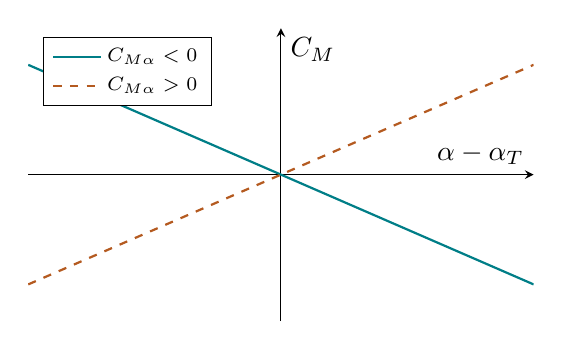
\begin{tikzpicture}
\begin{axis}[width=8cm,height=5.3cm,xlabel={$\alpha-\alpha_T$},ylabel={$C_M$},axis lines=middle,xmin=-3,xmax=3,ymin=-1,ymax=1,xtick={0},ytick={0},legend style={font=\scriptsize,at={(.03,.97)},anchor=north west}]
\addplot[teal,thick,domain=-3:3]{-.25*x};\addlegendentry{$C_{M\alpha}<0$}
\addplot[orange,thick,dashed,domain=-3:3]{.25*x};\addlegendentry{$C_{M\alpha}>0$}
\end{axis}
\end{tikzpicture}
\end{column}
\begin{column}{.4\textwidth}
\bi\item 零力矩交點表示配平。
\item 斜率表示初始恢復能力。
\item 更陡的負斜率通常代表更大的靜恢復作用。
\item 此圖沒有時間軸，不能直接讀取阻尼或收斂時間。\ei
\end{column}
\end{columns}
}
\slide{中性點與靜裕度}{3.3.1，pp. 111--112}{
\[SM=\frac{x_{NP}-x_{CG}}{c}\]
此處位置沿機身向後為正。$NP$ 為使 $C_{M\alpha}=0$ 的 CG 位置，也稱中性點。
\bi
\item CG 在中性點前方：$SM>0$，對應教材的縱向靜穩定配置。
\item CG 向後移動，靜裕度下降。越過中性點就失去自然縱向靜穩定。
\item 教材例子：$SM=10\%$、$c=4\ \mathrm{m}$，CG 往後移 $0.4\ \mathrm{m}$ 會到達中性點。
\ei
\key{補充關係}簡化線性模型中，$C_{M\alpha}=-C_{L\alpha}SM$。升力斜率與中性點必須對應同一整機模型及操縱面約束。
}
\originalfigure{3.11}{陣風與自然恢復力矩}{113}{fig-3-11.png}{比較向上陣風、配平及向下陣風時，迎角與恢復力矩的方向。}{}

\slide{不穩定配置與主動穩定}{3.3.2，pp. 112--114}{
\bi
\item 教材比較的配置將 CG 放在整機氣動中心後方，尾翼可向上提供配平升力。
\item 主翼所需升力減少，迎角與升力相關阻力可能下降。尾翼容積也可能縮小，但仍受起飛旋轉等要求限制。
\item 代價是失去自然恢復趨勢，需要感測器、計算器和致動器持續閉迴路控制。
\item 教材指出高機動不穩定戰機的擾動振幅倍增時間可能短至約 0.25 秒，超過飛行員可持續補償的能力。
\ei
\key{補充計算}若振幅按 $e^{\lambda t}$ 增長，$t_2=\ln2/\lambda$。$t_2=0.25\ \mathrm{s}$ 對應 $\lambda\approx2.77\ \mathrm{s^{-1}}$。
}
\originalfigure{3.12}{不穩定飛機的配平配置}{113}{fig-3-12.png}{注意 CG 與氣動中心的相對位置，以及尾翼升力的方向。}{}

\originalfigure{3.13}{倒著騎自行車的控制類比}{114}{fig-3-13.png}{教材用此圖說明不穩定配置需要快速、持續的修正。}{}

\originalfigure{3.14}{Tornado 與 FBW Jaguar}{115}{fig-3-14.png}{教材以編隊照片比較配平尾翼力方向不同的兩種配置。}{Photo: Arthur Gibson / British Aerospace Defence Ltd.}

\slide{整機穩定性不只由機翼決定}{3.3.3，p. 114；本單元自我檢查}{
\bi
\item 機身也產生升力與側向力，力的作用位置會影響俯仰與偏航穩定性。
\item 吊艙式發動機外罩也可能產生顯著氣動力，不能只把它當作重量。
\item 分析需要使用整機導數，不能直接以孤立機翼資料替代。
\ei
\key{自我檢查}
\begin{enumerate}
\item $C_M=0$ 足以判定穩定？\quad\textbf{否，還須看斜率與完整動態。}
\item CG 後移通常如何影響靜裕度？\quad\textbf{使其減小。}
\item 更大的負 $C_{M\alpha}$ 保證較大阻尼？\quad\textbf{否，恢復與阻尼是不同作用。}
\end{enumerate}
}

\section{3.4 運動方程與氣動導數}
\slide{六自由度與機體座標}{3.4.1，pp. 115--116}{
\small
原點設在 CG，$x$ 朝前、$y$ 朝右翼、$z$ 朝下，採右手座標系。
\begin{center}\begin{tabular}{ccccc}
\toprule 軸 & 平移速度 & 角速度 & 力 & 力矩\\\midrule
$x$ & $U$ & $p$：roll & $X$ & $L$\\
$y$ & $V$ & $q$：pitch & $Y$ & $M$\\
$z$ & $W$ & $r$：yaw & $Z$ & $N$\\\bottomrule
\end{tabular}\end{center}
\bi\item 正 $p$ 為右翼下降，正 $q$ 為抬頭，正 $r$ 為機頭向右。
\item 機體座標適合短期控制模型，也與機載陀螺儀、加速度計的量測軸一致。
\item 地理／慣性座標適合描述航跡與導航。兩者需透過姿態轉換連接。\ei
}
\originalfigure{3.15}{機體軸、速度與操縱面}{116}{fig-3-15.png}{對照軸向、角速度與控制面符號，尤其注意 z 軸朝下。}{}

\slide{旋轉座標系中的加速度}{3.4.1，pp. 116--117，式 (3.13)--(3.15)}{
\[\mathbf a_B=\dot{\mathbf V}_B+\boldsymbol\omega_B\times\mathbf V_B,
\qquad\mathbf V_B=\begin{bmatrix}U\\V\\W\end{bmatrix},\quad
\boldsymbol\omega_B=\begin{bmatrix}p\\q\\r\end{bmatrix}.\]
\[\begin{aligned}
a_x&=\dot U-Vr+Wq,\\
a_y&=\dot V+Ur-Wp,\\
a_z&=\dot W-Uq+Vp.
\end{aligned}\]
\key{物理意義}機體座標本身會旋轉。即使速度分量瞬間不變，速度向量在慣性空間仍可能改變方向，所以不能只用 $\dot U,\dot V,\dot W$ 表示加速度。
}
\originalfigure{3.16}{座標旋轉造成的速度變化}{117}{fig-3-16.png}{將圖上的微小向量變化連到角速度與速度向量的叉積項。}{}

\slide{Euler 角與旋轉次序}{3.4.2，pp. 118--119}{
\bi
\item 姿態以偏航 $\psi$、俯仰 $\theta$、滾轉 $\phi$ 描述，依序施加 yaw、pitch、roll 旋轉。
\item 三維旋轉通常不可交換次序。相同三個角度，改變次序會得到不同姿態。
\item 陀螺儀量到的是機體角速度 $p,q,r$，一般不等於 Euler 角變化率。
\ei
\[\begin{aligned}
p&=\dot\phi-\dot\psi\sin\theta,\\
q&=\dot\theta\cos\phi+\dot\psi\cos\theta\sin\phi,\\
r&=\dot\psi\cos\theta\cos\phi-\dot\theta\sin\phi.
\end{aligned}\]
}
\originalfigure{3.17}{Euler 姿態角}{118}{fig-3-17.png}{區分姿態角與機體角速度，並留意旋轉次序的重要性。}{}

\slide{Euler 角速度的反解}{3.4.2，p. 119；補充代數反解}{
\[\begin{bmatrix}\dot\phi\\\dot\theta\\\dot\psi\end{bmatrix}
=\begin{bmatrix}
1&\sin\phi\tan\theta&\cos\phi\tan\theta\\
0&\cos\phi&-\sin\phi\\
0&\sin\phi/\cos\theta&\cos\phi/\cos\theta
\end{bmatrix}\begin{bmatrix}p\\q\\r\end{bmatrix}.\]
\bi
\item 近水平、小角度擾動下，$\dot\phi\simeq p$、$\dot\theta\simeq q$、$\dot\psi\simeq r$。
\item 大坡度轉彎時，$q$ 會含偏航角變化的投影，不能直接令 $q=\dot\theta$。
\item $\cos\theta=0$ 使此組參數化奇異。這是 Euler 角描述的限制，並非飛機物理運動無法存在。
\ei
}
\slide{小擾動線性化的起點}{3.4.3，pp. 119--122}{
\[U=U_0+u,\qquad V=v,\qquad W=W_0+w.\]
\bi
\item 參考狀態為等速、平直、配平飛行，無側滑與角速度。$u,v,w,p,q,r$ 為偏離此狀態的小量。
\item 捨棄二階小量乘積，例如 $vr,uq,wp$。保留 $U_0r,W_0q$，因為 $U_0,W_0$ 是參考值。
\item $W_0$ 不必為零：機體 $x$ 軸若未與速度向量重合，配平速度仍有 $z$ 軸分量。
\item 模型只在指定配平點附近成立。高度、速度、Mach 數或構型改變時，係數也會改變。
\ei
}
\originalfigure{3.18}{飛機受到的外力}{120}{fig-3-18.png}{配平時各方向的合力為零，擾動模型處理的是力的增量。}{}

\slide{小擾動力與力矩方程}{3.4.3，pp. 121--122，式 (3.22)--(3.27)}{
\small
扣除配平狀態的合力與合力矩，且配平俯仰角很小時：
\[\begin{aligned}
X_a-mg\theta&=m(\dot u+W_0q),\\
Y_a+mg\phi&=m(\dot v-W_0p+U_0r),\\
Z_a&=m(\dot w-U_0q).
\end{aligned}\]
\[L=I_x\dot p,\qquad M=I_y\dot q,\qquad N=I_z\dot r.\]
\bi
\item $-mg\theta$ 與 $mg\phi$ 來自重力在旋轉後機體軸上的分量變化。
\item 角運動式採教材的主慣性軸近似，使慣性積為零，並忽略角速度乘積。
\item 只有左右對稱，不足以保證任選機體軸的 $I_{xz}$ 必定為零。\ei
}
\originalfigure{3.19}{氣動力、推力與重力分量}{121}{fig-3-19.png}{對照重力投影與三軸力矩，核對運動方程中的符號。}{}

\slide{氣動導數就是局部偏導數}{3.4.4，pp. 122--123}{
\[\Delta F\simeq\sum_i\left.\frac{\partial F}{\partial x_i}\right|_{\rm trim}\Delta x_i.\]
例如 $X_u=\partial X/\partial u$，表示其他變數固定時，前向速度小幅改變造成的 $x$ 方向力變化率。
\[X_a\simeq X_u u+X_w w,\qquad M\simeq M_w w+M_q q+M_\eta\eta+\cdots\]
\bi
\item 下標指出「對哪個變數微分」，前面的字母指出「哪種力或力矩」。
\item 導數必須在指定飛行狀態、構型與 CG 位置附近使用。
\item 各導數可由分析、試驗或辨識取得。局部線性不代表整個飛行包線都線性。
\ei
}
\slide{導數的單位與角度轉換}{3.4.4，pp. 123、130--131；補充單位檢查}{
\small
\begin{tabular}{lll}
\toprule 導數 & 定義 & 單位\\\midrule
$X_u$ & $\partial X/\partial u$ & $\mathrm{N/(m/s)}$\\
$M_w$ & $\partial M/\partial w$ & $\mathrm{N\,m/(m/s)}$\\
$M_q$ & $\partial M/\partial q$ & $\mathrm{N\,m/(rad/s)}$\\
$M_\eta$ & $\partial M/\partial\eta$ & $\mathrm{N\,m/rad}$\\
$M_\alpha$ & $\partial M/\partial\alpha$ & $\mathrm{N\,m/rad}$\\\bottomrule
\end{tabular}
\[w\simeq U_0\alpha\quad\Longrightarrow\quad M_\alpha=U_0M_w,\quad Z_\alpha=U_0Z_w.\]
上述轉換假設參考 $x$ 軸近似對準速度方向，且 $U_0$ 固定。
\key{常見錯誤}有的資料先以 $m$ 或 $I_y$ 除過導數，有的使用無因次導數。拿到數值前先核對定義，避免重複除以慣性或漏掉尺度。
}
\slide{縱向導數：速度與迎角的作用}{3.4.4.1，pp. 124--125}{
\small
\begin{tabular}{p{.22\textwidth}p{.64\textwidth}}
\toprule 導數 & 物理來源\\\midrule
$X_u,\ Z_u$ & 速度改變動壓與氣動係數，使阻力、升力改變。\\
$X_w,\ Z_w$ & 垂直速度擾動改變迎角，進而改變升力與阻力。\\
$M_w$ & 迎角擾動引起俯仰力矩，是縱向靜穩定的重要指標。\\
$M_u$ & 速度改變引起俯仰力矩。教材視為相對小而省略。\\\bottomrule
\end{tabular}
\key{方向判斷}在 $z$ 向下、正迎角增加升力的慣例下，通常 $Z_w<0$。穩定配置通常有 $M_w<0$。導數仍應以實際座標、操作點與構型判定。
}
\slide{俯仰阻尼的來源}{3.4.4.1，p. 125，圖 3.20}{
尾翼距離 CG 為 $l_t$。機體有俯仰角速度 $q$ 時，尾翼產生切向速度，其大小約為 $l_tq$。
\[\Delta\alpha_t\simeq\frac{l_tq}{V_T}\]
\bi
\item 這個局部氣流角度改變尾翼升力，尾翼力再乘上 $l_t$ 形成俯仰力矩。
\item 阻尼力矩通常反抗當前角速度，所以帶符號的 $M_q<0$。
\item $Z_q q$ 是同一現象造成的垂直力，$M_q q$ 是其俯仰力矩。
\ei
\key{恢復與阻尼}迎角誤差引起 $M_\alpha\alpha$，角速度引起 $M_q q$。前者像彈簧，後者像阻尼器。
}
\originalfigure{3.20}{俯仰率造成的尾翼阻尼}{125}{fig-3-20.png}{尾翼切向速度改變局部迎角，其力矩反抗原來的俯仰運動。}{}

\slide{下洗延遲與控制導數}{3.4.4.1，pp. 125--126}{
\bi
\item 機翼迎角改變後，下洗變化需經過一段傳遞時間才作用於尾翼。
\item 教材以 $Z_{\dot w}\dot w$、$M_{\dot w}\dot w$ 近似這種非定常效果。
\item 升降舵或全動尾翼偏轉 $\eta$，產生 $Z_\eta\eta$ 的垂直力與 $M_\eta\eta$ 的俯仰力矩。
\item $\eta$ 的正方向取決於操縱面定義，不能只靠「正舵角」三個字推測力矩方向。
\ei
\[\begin{aligned}
X_a&=X_u u+X_w w,\\
Z_a&=Z_u u+Z_w w+Z_{\dot w}\dot w+Z_q q+Z_\eta\eta,\\
M&=M_w w+M_q q+M_{\dot w}\dot w+M_\eta\eta.
\end{aligned}\]
}
\slide{側滑力與風向標穩定}{3.4.4.2，pp. 126--128}{
\bi
\item 側滑速度 $v$ 使機身側面與垂直尾翼受到側向氣流，產生側向力 $Y_vv$。
\item 垂直尾翼的側力乘上距 CG 的力臂，產生使機頭對準相對氣流的恢復力矩。
\item 機身側向氣動作用可能抵銷尾翼的穩定作用，因此要看整機的 $N_v$。
\item 垂尾面積與力臂的乘積形成 fin volume，也須滿足非對稱推力等控制需求。
\ei
\key{本筆記的側滑符號}
後續狀態模型採 $\beta\simeq v/U_0$。在此慣例下，通常 $Y_v<0$、方向穩定時 $N_v>0$。教材 p. 152 的純偏航角度約定將另行說明。
}
\originalfigure{3.21}{側滑與側向力}{127}{fig-3-21.png}{區分機身側力和垂尾側力，以及它們關於 CG 的力矩。}{}

\slide{側滑如何產生滾轉}{3.4.4.2，p. 128，圖 3.22}{
\bi
\item 上反角（dihedral）使側滑時左右翼的有效迎角不同，升力差產生 $L_vv$。
\item 後掠翼也會讓側滑改變左右翼受流狀況，即使幾何上反角為零，仍可有側滑滾轉效應。
\item 垂尾側力的作用點若在滾轉軸上方，也會產生滾轉力矩。
\item 機身繞流與高／低翼布局會改變此效果。教材指出低翼布局通常需較大的幾何上反角。
\ei
\key{理解重點}上反角主要透過「側滑」影響滾轉。只有坡度角本身，不能直接替代側滑角來計算 $L_vv$。
}
\originalfigure{3.22}{上反角與側滑的作用}{128}{fig-3-22.png}{側滑改變左右翼有效迎角，升力差因而產生滾轉力矩。}{}

\slide{角速度導數與橫向耦合}{3.4.4.2，pp. 128--129}{
\small
\begin{tabular}{p{.16\textwidth}p{.71\textwidth}}
\toprule 項 & 形成機制\\\midrule
$L_pp$ & 滾轉造成左右翼垂直速度不同，形成反抗滾轉的升力差。通常 $L_p<0$。\\
$N_pp$ & 滾轉造成左右翼升力與阻力差，進而產生偏航力矩。\\
$N_rr$ & 偏航使垂尾產生局部側向速度，形成反抗偏航的力矩。通常 $N_r<0$。\\
$L_rr$ & 偏航使左右翼相對氣流速度不同，升力差造成滾轉力矩。\\\bottomrule
\end{tabular}
\key{為何要保留耦合}副翼引起的滾轉會影響偏航，偏航又影響側滑與滾轉，因此真實橫向響應不只有一個滾轉時間常數。
}
\originalfigure{3.23}{滾轉率造成的阻尼力矩}{129}{fig-3-23.png}{比較左右翼的局部速度與升力變化，辨認反抗滾轉的力矩。}{}

\slide{副翼與方向舵的控制導數}{3.4.4.2，pp. 129--130}{
\small
$\xi$ 為差動副翼偏轉，$\zeta$ 為方向舵偏轉。
\bi
\item $L_\xi$：副翼造成升力差，直接控制滾轉。
\item $N_\xi$：副翼伴隨阻力差，造成偏航耦合，可能需要方向舵協調。
\item $Y_\zeta,N_\zeta$：方向舵造成側向力與偏航力矩。
\item $L_\zeta$：方向舵側力等效作用高度等因素帶來滾轉力矩。
\ei
\[\begin{aligned}
Y_a&=Y_vv+Y_\zeta\zeta,\\
L&=L_vv+L_pp+L_rr+L_\xi\xi+L_\zeta\zeta,\\
N&=N_vv+N_pp+N_rr+N_\xi\xi+N_\zeta\zeta.
\end{aligned}\]
}
\slide{縱向與橫向何時可以分開？}{3.4.4--3.4.5，pp. 123--131}{
\bi
\item 對稱飛機、對稱的平直配平狀態，以及小擾動線性化，使縱向與橫向可以近似解耦。
\item 縱向組：前向速度 $u$、垂直速度 $w$、俯仰角速度 $q$ 與姿態 $\theta$。
\item 橫向組：側滑速度 $v$、滾轉角速度 $p$、偏航角速度 $r$ 與坡度 $\phi$。
\item 大迎角、大幅度動作、非對稱掛載、強耦合或非對稱配平時，此分法可能不足。
\ei
\key{階數提醒}「三條動力學方程」不代表模型一定只有三個狀態。加入姿態運動學方程後，常見模型為四階。
}
\slide{完整線性縱向方程}{3.4.5，p. 131，式 (3.34)--(3.36)}{
\small
\[\begin{aligned}
m\dot u&=X_u u+X_w w-mW_0q-mg\theta,\\
(m-Z_{\dot w})\dot w&=Z_u u+Z_w w+(mU_0+Z_q)q+Z_\eta\eta,\\
I_y\dot q-M_{\dot w}\dot w&=M_w w+M_q q+M_\eta\eta,\\
\dot\theta&=q.
\end{aligned}\]
\bi
\item $\dot w$ 同時出現在垂直力與俯仰力矩方程，要先聯立整理，才能寫成標準狀態空間。
\item 可先寫成 $E\dot{\mathbf x}=A_0\mathbf x+B_0\eta$，若 $E$ 可逆，再求 $A=E^{-1}A_0$。
\item 教材後續示範會省略 $Z_q,Z_{\dot w},M_{\dot w}$，得到較清楚的四階矩陣。
\ei
}
\slide{縱向狀態空間模型}{3.4.5，pp. 131--133，式 (3.40)、(3.42)}{
\small
\[\mathbf x_\ell=\begin{bmatrix}u&w&q&\theta\end{bmatrix}^{T},
\qquad\dot{\mathbf x}_\ell=A_\ell\mathbf x_\ell+B_\ell\eta\]
\[A_\ell=\begin{bmatrix}
X_u/m&X_w/m&-W_0&-g\\
Z_u/m&Z_w/m&U_0&0\\
0&M_w/I_y&M_q/I_y&0\\
0&0&1&0
\end{bmatrix},\qquad
B_\ell=\begin{bmatrix}0\\Z_\eta/m\\M_\eta/I_y\\0\end{bmatrix}.\]
\bi
\item 最後一列為姿態運動學。$-g\theta$ 將姿態變化連接回前向速度。
\item $A$ 描述飛機自身動態，$B$ 描述控制輸入如何驅動狀態。
\item 矩陣中特定零元素來自本模型的省略，不是所有飛機都恆為零。
\ei
}
\slide{橫向狀態空間模型}{3.4.5，pp. 132--134，式 (3.41)、(3.43)}{
\small
\[\mathbf x_t=\begin{bmatrix}v&p&r&\phi\end{bmatrix}^{T},
\quad\mathbf u_c=\begin{bmatrix}\zeta&\xi\end{bmatrix}^{T}\]
\[\dot{\mathbf x}_t=
\begin{bmatrix}
Y_v/m&W_0&-U_0&g\\
L_v/I_x&L_p/I_x&L_r/I_x&0\\
N_v/I_z&N_p/I_z&N_r/I_z&0\\
0&1&0&0
\end{bmatrix}\mathbf x_t+
\begin{bmatrix}
Y_\zeta/m&0\\
L_\zeta/I_x&L_\xi/I_x\\
N_\zeta/I_z&N_\xi/I_z\\
0&0
\end{bmatrix}\mathbf u_c.\]
\key{物理對照}第一列含側力、旋轉座標項與重力側向分量。第二、三列相互耦合。最後一列是 $\dot\phi=p$。
}
\slide{由模型計算響應與模態}{3.4.5，pp. 132--134；補充特徵值觀點}{
\[\dot{\mathbf x}=A\mathbf x+B\mathbf u_c,\qquad
\mathbf x_{k+1}\simeq\mathbf x_k+\Delta t(A\mathbf x_k+B\mathbf u_{c,k}).\]
\bi
\item 教材用前向 Euler 法說明數值積分。$\Delta t$ 必須足夠小，並檢查縮小步長後結果是否收斂。
\item 自由響應的模態由 $A$ 的特徵值決定。負實部表示衰減，正實部表示發散。
\item 複數共軛根表示振盪。虛部決定振盪頻率，實部決定包絡衰減率。
\item 若輸出為 $y=C\mathbf x$，零初值下 $G(s)=C(sI-A)^{-1}B$。這把狀態空間接到傳遞函數。
\ei
}
\slide{本單元自我檢查}{3.4，pp. 115--134}{
\begin{enumerate}\setlength{\itemsep}{8pt}
\item 為何保留 $U_0r$ 卻捨棄 $ur$？\\
\textbf{前者是一階擾動項，後者是兩個小量相乘。}
\item $M_w$ 與 $M_q$ 分別代表什麼？\\
\textbf{迎角／垂直速度帶來的恢復力矩，以及俯仰角速度帶來的阻尼力矩。}
\item 有側滑時，是否只需要一條側向力方程？\\
\textbf{否，還會激發滾轉與偏航力矩。}
\item 不同飛行條件可否直接共用一組 $A,B$？\\
\textbf{只有局部近似合理時可以，否則須更新導數或採增益排程。}
\end{enumerate}
}

\section{3.5 縱向控制與響應}
\slide{升降舵輸入如何改變飛行路徑}{3.5.1，pp. 134--135}{
\bi
\item 升降舵／尾翼偏轉，先改變尾翼力與俯仰力矩。
\item 俯仰力矩使 $q$ 增加，機身旋轉使迎角改變，主翼升力隨之改變。
\item 新的升力提供使航跡彎曲的法向力。恢復力矩與俯仰阻尼限制響應。
\item 慣性使響應可能有過衝。固定輸入在短週期定速近似下，可對應近似固定的 $q$ 與迎角增量。
\ei
\key{精確一點}小角度下 $\alpha\simeq\theta-\gamma$，所以 $\dot\gamma=q-\dot\alpha$。只有迎角變化很慢時，航跡曲率加速度才近似 $a_n\simeq Uq$。
}
\originalfigure{3.24}{縱向機動的建立過程}{135}{fig-3-24.png}{從尾翼力矩、迎角變化，依序追到主翼升力與航跡彎曲。}{}

\slide{桿力每 g 與人工力感}{3.5.2，pp. 135--136}{
\bi
\item 動壓越高，相同迎角增量所產生的升力通常越大，因此每 $g$ 所需舵角與桿位移改變。
\item 教材指出高性能飛機的 stick displacement/$g$ 可能跨包線變化達約 40:1。
\item 純手動操縱時，飛行員可感到氣動鉸鏈力矩。全動力操縱隔離此力感，需要人工力感裝置。
\item 簡單彈簧提供桿力與位移關係；較完整的人工力感裝置依動壓調整剛度。
\ei
\key{設計目的}讓飛行員施力與希望得到的機動程度有可預期的關係，同時讓響應與阻尼在包線內維持可接受程度。
}
\slide{完整縱向響應的兩個時間尺度}{3.5.3，pp. 136--138}{
\[\frac{q(s)}{\eta(s)}
=\frac{K(s^3+b_2s^2+b_1s+b_0)}
{s^4+a_3s^3+a_2s^2+a_1s+a_0}\]
\bi
\item 典型穩定縱向模型可呈現兩對複數極點，分別對應短週期與長週期運動。
\item 短週期：迎角、俯仰角速度明顯變化，速度來不及大幅變動。教材典型週期約 1--10 秒。
\item 長週期（phugoid）：高度與速度交換位能和動能，迎角近似不變。教材列舉約 40 秒到數分鐘。
\item 這是典型模態描述，不保證所有操作點都恰好有兩對穩定複數根。
\ei
}
\originalfigure{3.25}{短週期與長週期響應}{138}{fig-3-25.png}{上方是俯仰率，下方是尾翼輸入，留意兩種時間尺度。}{}

\slide{短週期近似的假設}{3.5.4，pp. 138--140}{
\bi
\item 前向速度 $U$ 近似常數，因此省略慢變的前向速度狀態。
\item 使用對準配平速度方向的穩定軸。小擾動時 $\alpha=w/U$。
\item 省略 $Z_{\dot w},M_{\dot w},Z_q$。先保留直接尾翼力 $Z_\eta\eta$，稍後再說明省略的效果。
\item 求解的狀態為迎角 $\alpha$ 和俯仰角速度 $q$，因此得到二階模型。
\ei
\[\begin{aligned}
\dot\alpha&=\frac{Z_\alpha}{mU}\alpha+q+\frac{Z_\eta}{mU}\eta,\\
\dot q&=\frac{M_\alpha}{I_y}\alpha+\frac{M_q}{I_y}q+\frac{M_\eta}{I_y}\eta.
\end{aligned}\]
}
\originalfigure{3.26}{穩定軸下的縱向力與力矩}{139}{fig-3-26.png}{核對迎角、俯仰率與尾翼偏轉在受力圖中的作用。}{}

\slide{正負號統一：帶符號導數與正大小值}{3.5.4，pp. 139--144；核對整理}{
教材先使用帶符號導數，方塊圖推導時又把恢復／阻尼項當正大小值。為避免混用，本筆記定義
\[a=-\frac{Z_\alpha}{mU}>0,\qquad b=-\frac{M_q}{I_y}>0,\qquad
c=-\frac{M_\alpha}{I_y}>0,\qquad d=\frac{M_\eta}{I_y}.\]
這裡 $a,b,c>0$ 對應常見靜穩定、有阻尼配置，並選 $\eta$ 正向使 $d>0$。
\[\boxed{\dot\alpha=-a\alpha+q+e\eta,\qquad
\dot q=-c\alpha-bq+d\eta},\qquad e=\frac{Z_\eta}{mU}.\]
\key{好處}負號直接寫在方程中。$a,b,c$ 的值與正方向有清楚定義，後續不再把負導數誤代入正時間常數。
}
\originalfigure{3.27}{俯仰運動的方塊圖}{140}{fig-3-27.png}{保留教材原符號；求和點的負號與導數大小值須搭配前頁約定閱讀。}{}

\originalfigure{3.28}{迎角運動的方塊圖}{141}{fig-3-28.png}{觀察俯仰率、直接尾翼力與迎角回授如何共同影響迎角變化率。}{}

\slide{消去迎角，得到俯仰角速度傳遞函數}{3.5.4，式 (3.44)--(3.60)；補充一致推導}{
依教材簡化，先令 $e=0$，在零初始條件下取 Laplace 轉換：
\[(s+a)\alpha=q,\qquad (s+b)q=-c\alpha+d\eta.\]
代入第一式：
\[\big[(s+a)(s+b)+c\big]q=d(s+a)\eta.\]
因此
\[\boxed{\frac q\eta=\frac{d(s+a)}{s^2+(a+b)s+ab+c}},\qquad
\boxed{\frac\alpha\eta=\frac{d}{s^2+(a+b)s+ab+c}}.\]
\key{物理意義}兩個輸出共享同一組極點，但 $q/\eta$ 多一個零點 $s=-a$，所以兩種輸出的過衝與波形並不相同。
}
\originalfigure{3.29}{一般負回授關係}{141}{fig-3-29.png}{辨認前向路徑與回授路徑，再將此關係套用到飛機內部動態。}{}

\slide{保留直接尾翼力時會改變什麼？}{3.5.4，p. 142；補充推導}{
保留 $e=Z_\eta/(mU)$：
\[(s+a)\alpha=q+e\eta,\qquad(s+b)q=-c\alpha+d\eta.\]
\[\frac q\eta=\frac{d(s+a)-ce}{s^2+(a+b)s+ab+c},\qquad
\frac\alpha\eta=\frac{d+e(s+b)}{s^2+(a+b)s+ab+c}.\]
\bi
\item 在此固定狀態模型下，直接控制力改變分子，因而改變零點與強迫響應。
\item 分母不變，所以無輸入的自然模態不變。
\item 教材說它不影響自然穩定性，不能延伸理解成「它不會改變階躍過衝或輸入響應」。
\ei
}
\slide{與教材時間常數寫法的對照}{3.5.4，pp. 142--144}{
\[\begin{gathered}
T_1=\frac1b,\quad T_2=\frac1a,\quad K=da=\frac{d}{T_2},\\
A_1=a+b=\frac1{T_1}+\frac1{T_2},\qquad
A_2=ab+c=\frac1{T_1T_2}+c.
\end{gathered}\]
\[\frac q\eta=\frac{K(1+T_2s)}{s^2+A_1s+A_2},\qquad
\frac\alpha\eta=\frac{KT_2}{s^2+A_1s+A_2}.\]
\key{用帶符號導數計算時}
\[T_1=-\frac{I_y}{M_q},\quad T_2=-\frac{mU}{Z_\alpha},\quad
A_2=\frac{M_qZ_\alpha}{I_ymU}-\frac{M_\alpha}{I_y}.\]
}
\originalfigure{3.30}{簡化後的縱向回授模型}{142}{fig-3-30.png}{兩個一階環節與迎角恢復回授，構成短週期二階動態。}{}

\originalfigure{3.31}{俯仰率與迎角的傳遞關係}{143}{fig-3-31.png}{原圖以 D 表示微分算子；俯仰率與迎角共享極點，但零點不同。}{}

\slide{二階極點、自然頻率與阻尼比}{3.5.4，pp. 143--145}{
為免與方向舵角 $\zeta$ 混淆，本筆記用 $\zeta_d$ 表示阻尼比。
\[s^2+A_1s+A_2=s^2+2\zeta_d\omega_ns+\omega_n^2\]
\[\omega_n=\sqrt{A_2},\qquad\zeta_d=\frac{A_1}{2\sqrt{A_2}},\qquad
s_{1,2}=-\frac{A_1}{2}\pm\sqrt{\frac{A_1^2}{4}-A_2}.\]
\bi
\item 漸近穩定：$A_1>0$ 且 $A_2>0$。
\item $0<\zeta_d<1$：欠阻尼，$\omega_d=\omega_n\sqrt{1-\zeta_d^2}$。
\item $\zeta_d=1$：臨界阻尼。$\zeta_d>1$：過阻尼。
\item 靜不穩定時 $c<0$，若 $ab+c<0$，二階模型必有一個正實根。須以係數判斷，不能只看一個導數。
\ei
}
\originalfigure{3.32}{二階系統的自由響應}{145}{fig-3-32.png}{這張原圖是初始擾動的自由響應，不能直接當作所有輸出的階躍過衝圖。}{}

\slide{穩態增益與短週期模型的界線}{3.5.4，p. 144}{
對穩定的簡化模型，令時間導數為零：
\[q_{\rm ss}=\frac{K}{A_2}\eta_{\rm ss},\qquad
\alpha_{\rm ss}=\frac{KT_2}{A_2}\eta_{\rm ss}.\]
\bi
\item 相同尾翼偏轉所造成的穩態俯仰率，會隨導數、速度與密度改變。
\item $q_{\rm ss}\ne0$ 意味著姿態仍在變化，不能把這個「穩態」解讀成飛機永久保持新的固定姿態。
\item 這是定速短週期近似中的局部機動結果。長時間飛行仍須恢復速度、重力投影與航跡動態。
\ei
\key{控制連結}只改善極點不保證操縱增益不變。設計增穩系統也要檢查每單位桿位移產生多少機動。
}
\slide{短週期算例：已知資料與近似}{3.5.5，pp. 145--146}{
\small
\begin{tabular}{ll}
\toprule 參數 & 教材給定值\\\midrule
質量、速度 & $m=25{,}000\ \mathrm{kg}$，$U=250\ \mathrm{m/s}$\\
俯仰慣性矩 & $I_y=6\times10^5\ \mathrm{kg\,m^2}$\\
恢復力矩導數大小 & $\lvert M_\alpha\rvert=2\times10^7\ \mathrm{N\,m/rad}$\\
尾翼力臂 & $l_t=8\ \mathrm{m}$\\
每 $g$ 迎角、舵角增量 & $1.6^\circ/g$、$1^\circ/g$\\\bottomrule
\end{tabular}
\bi
\item 教材資料為代表性估算，並非某一特定真實飛機的完整識別模型。
\item 為重現書中步驟，先使用 $g\simeq10\ \mathrm{m/s^2}$、$1^\circ\simeq1/60\ \mathrm{rad}$。
\item 以下先使用恢復、阻尼的正大小值，與前面的 $a,b,c,d$ 定義一致。
\ei
}
\slide{短週期算例：由每 g 資料估計導數}{3.5.5，pp. 146--147}{
\small
$1.6^\circ$ 迎角增量產生 $1g$ 的升力增量：
\[\lvert Z_\alpha\rvert\frac{1.6}{60}=10m,\qquad
\lvert Z_\alpha\rvert=375m,\qquad
T_2=\frac{mU}{\lvert Z_\alpha\rvert}\simeq0.67\ \mathrm{s}.\]
全動尾翼近似下，俯仰角速度造成的局部迎角變化為 $l_tq/U$：
\[\lvert M_q\rvert\simeq\frac{l_t}{U}\lvert M_\eta\rvert
=0.032\lvert M_\eta\rvert.\]
$1g$ 機動約對應 $q=10/250=0.04\ \mathrm{rad/s}\simeq2.4^\circ/\mathrm{s}$，穩態力矩平衡為
\[\lvert M_\eta\rvert(1)
=(2\times10^7)(1.6)+(0.032\lvert M_\eta\rvert)(2.4).\]
各角度在同一式中統一用度表示，共同的弧度換算因子約去。
}
\slide{短週期算例：逐項重算係數}{3.5.5，p. 147；核對計算}{
\small
沿用教材四捨五入後的導數：
\[\lvert M_\eta\rvert\simeq3.5\times10^7,\quad
\lvert M_q\rvert\simeq1.1\times10^6,\quad T_1\simeq0.55\ \mathrm{s}.\]
\[\begin{aligned}
A_1&=\frac1{0.55}+\frac1{0.67}=\boxed{3.3107\ \mathrm{s^{-1}}},\\
A_2&=\frac{2\times10^7}{6\times10^5}+\frac1{0.55(0.67)}
=\boxed{36.0470\ \mathrm{s^{-2}}},\\
K&=\frac{3.5\times10^7}{6\times10^5(0.67)}=\boxed{87.0647\ \mathrm{s^{-3}}}.
\end{aligned}\]
\key{已確認的算術問題}教材印成 $A_1=2.3$。前一行的數值相加應為 3.31，差異並非一般四捨五入所致。
}
\slide{短週期算例：教材值與重算值}{3.5.5，pp. 147--148}{
\small
\begin{tabular}{lcc}
\toprule 量 & 教材後續採用 & 依前頁資料重算\\\midrule
$A_1$ & 2.3 & 3.3107\\
$A_2$ & 36 & 36.0470\\
$\omega_n$ & $6\ \mathrm{rad/s}$ & $6.0039\ \mathrm{rad/s}$\\
$\zeta_d$ & 約 0.2 & 0.2757\\
分母極點 & 約 $-1.15\pm j5.89$ & $-1.6554\pm j5.770$\\\bottomrule
\end{tabular}
\[\frac q\eta\simeq
\frac{87.0647(1+0.67s)}{s^2+3.3107s+36.0470}.\]
\key{理解}頻率變化不大，但阻尼比有明顯差異。後面的 SAS 增益估計也會跟著改變。
}
\slide{過衝公式的適用範圍}{3.5.4--3.5.5，pp. 144--148；補充核對}{
標準二階、無零點、單位 DC 增益、零初值的階躍響應：
\[G_0(s)=\frac{\omega_n^2}{s^2+2\zeta_d\omega_ns+\omega_n^2},
\qquad
M_p=e^{-\pi\zeta_d/\sqrt{1-\zeta_d^2}}.\]
\bi
\item $\zeta_d=0.2$ 時，標準階躍過衝約 $52.7\%$。
\item 重算的 $\zeta_d=0.2757$ 對應標準過衝約 $40.6\%$。
\item 簡化 $\alpha/\eta$ 無零點，歸一化後可使用此公式。
\item $q/\eta$ 有零點 $s=-1/T_2$，不能直接用同一公式推論俯仰率過衝。自由擾動響應還會依初始條件而變。
\ei
}
\slide{同一組極點，兩種不同階躍響應}{3.5.5；依重算模型作圖}{
\begin{columns}[T]
\begin{column}{.59\textwidth}
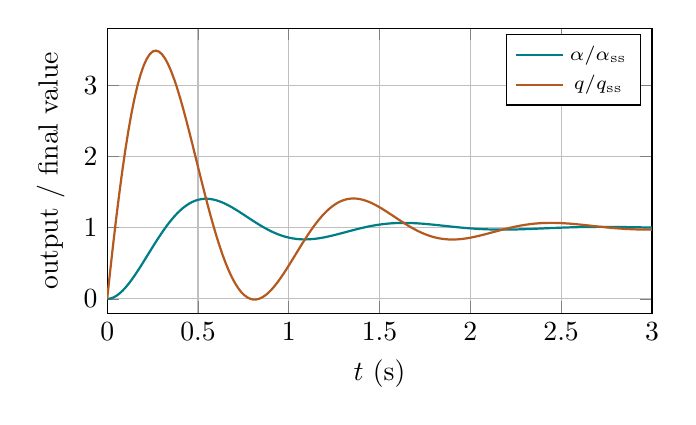
\begin{tikzpicture}
\begin{axis}[width=8.5cm,height=5.2cm,xlabel={$t\ (\mathrm{s})$},ylabel={output / final value},xmin=0,xmax=3,ymin=-.2,ymax=3.8,grid=major,legend style={font=\scriptsize}]
\addplot[teal,thick,domain=0:3,samples=180]{1-exp(-1.65536*x)*(cos(deg(5.7703*x))+1.65536/5.7703*sin(deg(5.7703*x)))};
\addlegendentry{$\alpha/\alpha_{\rm ss}$}
\addplot[orange,thick,domain=0:3,samples=180]{1+exp(-1.65536*x)*(-cos(deg(5.7703*x))+(36.047*.67-1.65536)/5.7703*sin(deg(5.7703*x)))};
\addlegendentry{$q/q_{\rm ss}$}
\end{axis}
\end{tikzpicture}
\end{column}
\begin{column}{.37\textwidth}
\small
零初值、小尾翼階躍，兩個輸出各自除以穩態值。
\bi\item 迎角峰值約 1.406。
\item 俯仰率峰值約 3.485，約出現在 0.267 秒。
\item 差別來自輸出零點，不是極點改變。
\item 這是簡化模型的響應，不代表真機實測。\ei
\end{column}
\end{columns}
}

\section{3.6 橫向控制}
\slide{坡度轉彎的力平衡}{3.6.1，pp. 148--149}{
考慮協調、等速、等高度轉彎。用 $L_{\rm lift}$ 表示總升力，避免與滾轉力矩 $L$ 混淆。
\[L_{\rm lift}\cos\phi=mg,\qquad
L_{\rm lift}\sin\phi=mV_T\dot\psi.\]
\[\boxed{\dot\psi=\frac{g\tan\phi}{V_T}},\qquad
\boxed{R=\frac{V_T^2}{g\tan\phi}},\qquad
\boxed{n=\frac{L_{\rm lift}}{mg}=\sec\phi}.\]
\bi
\item 升力的水平分量提供向心力，垂直分量仍須支撐重量。
\item 固定坡度時，速度越快，轉彎率越小、半徑越大。
\item 不能只增加坡度而不增加升力，否則會損失高度。
\ei
}
\originalfigure{3.33}{協調水平轉彎的受力}{149}{fig-3-33.png}{水平升力提供向心力，垂直分量平衡重量。}{}

\slide{轉彎算例與數值核對}{3.6.1，p. 149；補充計算}{
\small
$\phi=60^\circ$、$V_T=100\ \mathrm{m/s}$、$g=9.81\ \mathrm{m/s^2}$：
\[\begin{aligned}
n&=\sec60^\circ=2,\\
a_{\rm centripetal}&=g\tan60^\circ=1.732g,\\
\dot\psi&=\frac{9.81\tan60^\circ}{100}
=0.1699\ \mathrm{rad/s}=9.74^\circ/\mathrm{s},\\
R&\simeq588.5\ \mathrm{m}.
\end{aligned}\]
\key{核對提醒}教材列出的轉彎率為 $10.4^\circ/\mathrm{s}$。依同頁公式與 $100\ \mathrm{m/s}$ 重算得到約 $9.74^\circ/\mathrm{s}$。即使用 $g\simeq10$，也約為 $9.92^\circ/\mathrm{s}$。
}
\slide{協調轉彎需要哪些輸入？}{3.6.1，pp. 149--150}{
\bi
\item 副翼先建立滾轉角速度，到達所需坡度後將桿移回配平附近，以停止繼續滾轉。
\item 升降舵增加迎角與升力，以維持高度並產生所需向心力。
\item 方向舵修正副翼引起的偏航與側滑，使轉彎接近協調。
\item 油門增加推力以補償阻力增加，維持真空速。
\ei
\key{飛行員感受到的力}協調轉彎時，重力與慣性效果的合成感受大致沿機體法向，理想上沒有明顯側向滑動感。高 $g$ 轉彎仍需足夠升力與推力。
}
\slide{純滾轉的一階近似}{3.6.1，p. 150，式 (3.67)--(3.69)}{
忽略側滑與偏航耦合：
\[I_x\dot p=L_\xi\xi+L_pp,\qquad L_p<0.\]
\[\frac{p(s)}{\xi(s)}=\frac{L_\xi}{I_xs-L_p}
=\frac{K_R}{1+T_Rs},\quad
T_R=-\frac{I_x}{L_p}>0,\quad K_R=-\frac{L_\xi}{L_p}.\]
對階躍 $\xi_0$、零初值：
\[p(t)=K_R\xi_0(1-e^{-t/T_R}).\]
\key{核對提醒}保留導數正負號時，穩態增益必須為 $-L_\xi/L_p$。教材式 (3.68)--(3.69) 的正負號需要配合其大小值約定閱讀。
}
\originalfigure{3.34}{副翼階躍與滾轉率}{151}{fig-3-34.png}{將原圖的時間常數與漸近穩態值，對照一階響應公式。}{}

\slide{滾轉率與坡度是不同的輸出}{3.6.1，pp. 150--151；補充積分}{
\begin{columns}[T]
\begin{column}{.55\textwidth}
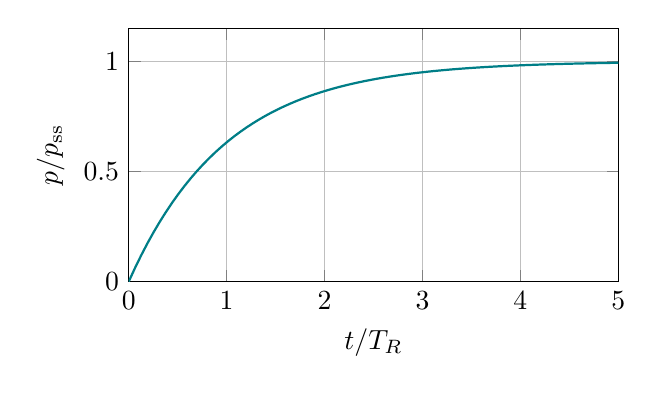
\begin{tikzpicture}
\begin{axis}[width=7.8cm,height=4.8cm,xlabel={$t/T_R$},ylabel={$p/p_{\rm ss}$},xmin=0,xmax=5,ymin=0,ymax=1.15,grid=major]
\addplot[teal,thick,domain=0:5,samples=80]{1-exp(-x)};
\end{axis}
\end{tikzpicture}
\end{column}
\begin{column}{.41\textwidth}
\small
\bi\item 一個時間常數後達穩態值的約 $63.2\%$。
\item 約 $3T_R$ 達 $95\%$。
\item 坡度為 $\phi(t)=\phi(0)+\int_0^t p(\tau)\,\dd\tau$。
\item 固定非零副翼在此模型中會持續滾轉，不會自動停在固定坡度。\ei
\end{column}
\end{columns}
}
\slide{方向舵的主要任務}{3.6.2，pp. 150--151}{
\bi
\item 修正副翼造成的偏航力矩，協助完成協調轉彎。
\item 抑制不希望出現的側滑，也能在需要時主動建立側滑。
\item 抵銷多發飛機單邊推力損失或非對稱外掛造成的偏航力矩。
\item 在側風落地的教材情境中，調整航向與跑道方向的對準關係。
\ei
\key{為何通常不用方向舵平轉？}機身與垂尾能提供的側向力遠小於主翼可提供的升力，且平轉會造成明顯側向加速度，效率與舒適性都較差。
}
\slide{純偏航模型的角度符號}{3.6.3，p. 152；核對角度約定}{
\small
以一般 $\beta=v/U$ 為側滑角，若速度向量的方向固定，而機頭向右偏航 $\psi>0$，則小角度下
\[\beta\simeq-\psi,\qquad v\simeq-U\psi.\]
所以在 $N_v>0$ 表示方向穩定的慣例下：
\[I_z\ddot\psi=N_v(-U\psi)+N_r\dot\psi,\qquad N_r<0,\]
\[\boxed{\ddot\psi+\frac{-N_r}{I_z}\dot\psi+\frac{N_vU}{I_z}\psi=0}.\]
\key{教材對照}教材寫 $\beta=\psi$ 並用 $N_v<0$ 表示恢復作用，這等效於另一個角度／導數正方向。不能把它與前面的 $v$ 慣例直接混用。
}
\slide{偏航振盪的自然頻率與阻尼}{3.6.3，pp. 152--153；一致符號推導}{
從前頁帶符號方程可得
\[\omega_{n,y}=\sqrt{\frac{N_vU}{I_z}},\qquad
\zeta_{d,y}=\frac{-N_r}{2\sqrt{I_zN_vU}}.\]
\bi
\item 垂尾恢復作用提供「剛度」，偏航慣性提供振盪的慣性，$N_r$ 提供阻尼。
\item 教材列舉純偏航振盪週期約 3--10 秒，阻尼不足時需要 yaw damper。
\item 教材的負 $N_v$ 慣例應改寫為 $\omega_n=\sqrt{-N_vU/I_z}$。同頁平方根式遺漏的符號不能照抄。
\item 若比較不同速度，必須同時更新 $N_v,N_r$。固定導數下的速度比例不能直接當作全包線規律。
\ei
}
\slide{Dutch roll、滾轉衰減與螺旋模態}{3.6.4，p. 153}{
\small
\begin{tabular}{p{.20\textwidth}p{.65\textwidth}}
\toprule 模態 & 物理描述\\\midrule
Dutch roll & 側滑、偏航與滾轉耦合的振盪。後掠與上反角效應影響各運動分量的比例。\\
Roll subsidence & 主要表現為滾轉率擾動快速衰減，常可用一階近似。\\
Spiral mode & 慢速的坡度、偏航與側滑演變，可能緩慢發散，教材例子時間尺度約半分鐘到一分鐘。\\\bottomrule
\end{tabular}
\key{相位提醒}教材用滾轉與偏航約相差 $90^\circ$ 作直觀描述。實際幅比與相位取決於模態特徵向量與觀測變數，不是所有飛機都精確相同。
}
\slide{橫向模型階數的核對}{3.4.5 與 3.6.4，pp. 133、153}{
\bi
\item p. 133 的 $\mathbf x=[v,p,r,\phi]^T$ 是四個狀態，因此 $\det(sI-A)$ 最高為四次。
\item 一般可用一對 Dutch roll 根，加上一個 roll 根與一個 spiral 根理解這個四階模型。
\item 若額外加入不回饋其他狀態的航向 $\dot\psi=r$，五階擴充模型會多一個零特徵值。
\item p. 153 列出五階分解，含另一個有限的 yaw subsidence 因子，與先前四階矩陣不能直接一一對上。
\ei
\key{使用原則}依實際採用的狀態方程計算極點。若要使用另一個五階模型，需先交代新增狀態與動態，不能只把五個模態硬套上四階矩陣。
}

\section{3.7 動力操縱與 PCU}
\slide{Power Control Unit 的作用}{3.7.1，pp. 154--155}{
\bi
\item 高速飛行時操縱面載荷很大，飛行員通常無法直接用人力驅動。
\item PCU 利用液壓能量產生大致動力，飛行員透過連桿移動小型伺服閥來發出命令。
\item 活塞移動透過機械回授逐漸關閉閥口，使活塞位置追隨輸入位置。
\item 教材的全動力系統要求避免操縱面反向驅動操縱機構，以處理回傳與顫振問題。
\ei
\key{能量與訊號}桿位移提供位置命令，液壓供應提供作動能量。機械傳令與液壓放大可以同時存在，並不等同於 FBW。
}
\originalfigure{3.35}{機械傳令的動力操縱系統}{154}{fig-3-35.png}{從飛行員操縱器沿連桿追到各操縱面的 PCU。}{Courtesy of BAE Systems.}

\slide{PCU 的力量與獨立供應}{3.7.1，p. 155}{
\bi
\item 教材典型液壓壓力約 $200\ \mathrm{bar}=20\ \mathrm{MPa}$。活塞面積決定可用力的尺度。
\item 兩套串聯致動結構與獨立液壓供應，用來提高失效後的控制能力。
\item 閥芯正常操縱力很小，但連桿仍可能需承受較大的人工作用力，以處理教材所述的卡閥情境。
\ei
\[F\simeq\Delta P\,A.\]
\key{補充算例}$\Delta P=20\ \mathrm{MPa}$、$A=10\ \mathrm{cm^2}=10^{-3}\ \mathrm{m^2}$ 時，$F\simeq20\ \mathrm{kN}$。這是面積與壓差的尺度估算，實際載荷須扣除回油壓與損失。
}
\slide{PCU 位置回授的幾何關係}{3.7.2，pp. 155--156，式 (3.72)}{
教材連桿幾何使閥口位移為
\[x_\varepsilon=\frac{x_i-Gx_o}{G+1}.\]
\bi
\item $x_i$：輸入桿位移。$x_o$：輸出活塞位移。$G$：教材定義的連桿比例。
\item 若輸入與回授尚未平衡，$x_\varepsilon\ne0$，液壓流動使活塞移動。
\item 理想穩態下，閥口重新關閉：$x_i-Gx_o=0$，所以 $x_o=x_i/G$。
\item 這是位置負回授，幾何比例決定 DC 增益，而液壓流量能力決定反應速度。
\ei
}
\originalfigure{3.36}{PCU 閥口與活塞回授}{155}{fig-3-36.png}{先辨認輸入、閥芯、液壓腔及活塞，再核對機械回授路徑。}{}

\slide{液壓流量如何形成一階模型}{3.7.2，pp. 156--157}{
\small
教材假設：方形且對稱的閥口、油液不可壓縮、外部負載與慣性可忽略、回油壓近似零。
\[a_{\rm port}=K_1x_\varepsilon,\qquad
v_{\rm oil}=K_2\sqrt{\Delta P}.\]
進出流量相等且活塞受力平衡時，
\[P_1=P_2=P_s/2,\qquad
Q_h=A\dot x_o=K_1K_2x_\varepsilon\sqrt{P_s/2}.\]
\[\dot x_o=K_vx_\varepsilon,\qquad K_v=\frac{K_1K_2}{A}\sqrt{\frac{P_s}{2}}.\]
\key{符號提醒}$Q_h$ 是液壓體積流率，與本章氣動壓力 $Q$ 不同。
}
\slide{PCU 傳遞函數、頻寬與相位}{3.7.2，p. 157，式 (3.73)--(3.75)}{
\[\dot x_o=\frac{K_v}{G+1}(x_i-Gx_o)\]
\[\boxed{\frac{x_o}{x_i}=\frac{1/G}{1+T_{\rm act}s}},
\qquad T_{\rm act}=\frac{G+1}{GK_v}.\]
\bi
\item 教材例子 $T_{\rm act}=0.1\ \mathrm{s}$，$-3\ \mathrm{dB}$ 頻率 $\omega_b=10\ \mathrm{rad/s}$，約 $1.59\ \mathrm{Hz}$。
\item $1\ \mathrm{Hz}$ 的相位為 $-\tan^{-1}(2\pi\cdot1\cdot0.1)\simeq-32.1^\circ$。
\item 致動器不是瞬間完成指令。相位延遲會降低外部飛控回路可用的穩定裕度。
\item 有負載、油液彈性、速率限制或間隙時，一階模型可能不足。
\ei
}

\section{3.8 穩定增強系統}
\slide{SAS 以回授建立額外阻尼}{3.8.1，pp. 157--158}{
\bi
\item 角速度感測器量測 $p,q,r$，控制器產生相對應的操縱面修正。
\item 修正輸入透過差動機構與飛行員命令相加，產生反抗角速度的附加力矩。
\item Pitch damper、roll damper、yaw damper 分別補充相應軸的阻尼。
\item Yaw damper 特別用於抑制 Dutch roll；強滾轉偏航耦合時，可能還需 roll damper。
\ei
\key{局部等效}若 $\eta=\delta_i-G_q q$ 且 $M_\eta>0$，則有效俯仰阻尼導數為 $M_{q,\rm eff}=M_q-M_\eta G_q$，變得更負。
}
\originalfigure{3.37}{簡單穩定增強系統}{158}{fig-3-37.png}{比較飛行員輸入和角速度回授如何在差動機構中合成。}{}

\slide{有限權限的意義}{3.8.1，p. 158}{
\bi
\item 有限權限 SAS 適合原本仍可飛、但部分包線阻尼不足的飛機。
\item 限制 SAS 的最大舵面修正量，可限制失效時造成的運動，使飛行員能解除並接手。
\item 教材給出的典型權限，相當於約 $\pm0.5g$ 的操縱面作用，但不同系統並非都採同一數值。
\item 單通道系統沒有平行備援，故失效安全依賴有限權限、可解除性與基本飛機的可控性。
\ei
\key{不能混淆}有限權限是「可施加多少控制」，單通道是「有幾條獨立鏈路」。兩者描述不同設計面向。
}
\slide{Wash-out 為何讓偏航阻尼器不抵抗轉彎？}{3.8.1，pp. 159--160}{
持續轉彎有非零的平均偏航率。若直接用純比例負回授，SAS 會試圖抵抗這個飛行員有意要求的轉彎。
\[
H_w(s)=\frac{T_ws}{1+T_ws}
\quad\text{（補充：典型洗出濾波器形式）}
\]
\bi
\item $H_w(0)=0$：穩態 DC 成分被去除。
\item 在目標振盪頻帶保留足夠角速度訊號，讓阻尼器針對振盪動作。
\item 再加高頻低通，例如 $1/(1+T_fs)$，形成低頻與高頻都衰減的頻率選擇。
\item 通帶仍可能有幅值與相位誤差，設計時要計算實際濾波器，不能假設一定零相移。
\ei
}
\originalfigure{3.38}{洗出與高頻截止的頻率特性}{159}{fig-3-38.png}{低頻抑制持續轉彎成分，高頻截止降低雜訊與結構模態的影響。}{}

\slide{結構模態、濾波與增益排程}{3.8.1，pp. 158--160}{
\bi
\item 致動器施力會使有限剛度的機體彎曲，陀螺儀可能量到彈性振動而不只是剛體轉動。
\item 若回授在結構頻率仍有足夠增益與不利相位，控制器可能激發該結構模態。
\item 低通抑制高頻訊號；notch filter 在特定結構共振附近提供較深的衰減。
\item 高度、速度改變會改變操縱效率，教材以切換兩三組增益說明簡單的增益排程。
\ei
\key{取捨}濾波抑制雜訊與共振，也會增加相位延遲。不能只以「濾得越多越好」決定控制器。
}
\slide{俯仰 SAS 的閉迴路推導}{3.8.1.1，pp. 160--161}{
\small
基本飛機模型與增穩律：
\[G_p(s)=\frac{K(1+T_2s)}{s^2+A_1s+A_2},\qquad
\eta=\delta_i-G_qq.\]
代入 $q=G_p(\delta_i-G_qq)$ 並整理：
\[\boxed{\frac q{\delta_i}=
\frac{K(1+T_2s)}
{s^2+(A_1+KT_2G_q)s+(A_2+KG_q)}}.\]
\[\omega_{n,\rm cl}^2=A_2+KG_q,\quad
2\zeta_{d,\rm cl}\omega_{n,\rm cl}=A_1+KT_2G_q.\]
\key{看係數的意義}速率回授同時改變阻尼係數與自然頻率，也改變 DC 增益 $K/(A_2+KG_q)$。這個推導仍忽略致動器、濾波器及感測器延遲。
}
\originalfigure{3.39}{俯仰率增穩回路}{161}{fig-3-39.png}{追蹤飛行員指令、俯仰率量測與增穩舵角的負回授。}{}

\slide{SAS 算例：教材的設計鏈}{3.8.1.1，p. 161}{
教材採用 $K=87$、$T_2=0.67$、$\omega_n=6$、$\zeta_d=0.2$，要求 $\zeta_{d,\rm cl}=0.7$：
\[
1.4\sqrt{36+87G_q}=2.4+87(0.67)G_q.
\]
\bi
\item 解得 $G_q$ 約 $0.12\ \mathrm{s}$，亦可寫成「度尾翼／（度每秒俯仰率）」。
\item 教材四捨五入後列出 $\omega_{n,\rm cl}\simeq6.8\ \mathrm{rad/s}$。
\item 閉迴路分母約為 $s^2+9.5s+46$。
\item 此設計沿用前面偏低的阻尼估計，故要與重算模型分開閱讀。
\ei
}
\slide{SAS 算例：依重算模型重新設計}{3.8.1.1；補充一致重算}{
\small
使用 $A_1=3.3107$、$A_2=36.0470$、$K=87.0647$，仍要求 $\zeta_{d,\rm cl}=0.7$：
\[
1.4\sqrt{36.0470+87.0647G_q}
=3.3107+87.0647(0.67)G_q.
\]
取符合原式且為正的解：
\[
\boxed{G_q=0.1045\ \mathrm{s}},\quad
\boxed{\omega_{n,\rm cl}=6.7190\ \mathrm{rad/s}}.
\]
\[
\frac q{\delta_i}\simeq
\frac{87.0647(1+0.67s)}
{s^2+9.4067s+45.1454}.
\]
\key{結果差異}重算的基本飛機原本阻尼較高，因此達到同樣目標需要的增穩增益較小。這個數值僅供理解本章簡化設計流程。
}
\slide{極點改善不等於所有輸出都同樣改善}{3.8.1.1，pp. 160--162；補充比較}{
\small
\begin{tabular}{lcc}
\toprule 量 & 重算的基本飛機 & 加入 $G_q=0.1045$\\\midrule
$\omega_n\ (\mathrm{rad/s})$ & 6.004 & 6.719\\
$\zeta_d$ & 0.276 & 0.700\\
$q$ 的 DC 增益 $(\mathrm{s^{-1}})$ & 2.415 & 1.929\\
約略包絡時間常數 $1/(\zeta_d\omega_n)$ & 0.604 s & 0.213 s\\\bottomrule
\end{tabular}
\bi
\item 衰減變快，但相同輸入的穩態俯仰率也降低了。
\item $q$ 通道的零點仍存在，不能把「阻尼比 0.7」直接翻譯為 $q$ 的固定過衝百分比。
\item 若致動器有顯著延遲，必須把其狀態納入閉迴路，再檢查穩定性。
\ei
}
\originalfigure{3.40}{加入增穩前後的響應}{162}{fig-3-40.png}{此圖為教材示意，用來比較振盪衰減，不當作本筆記重算模型的數值曲線。}{}

\slide{全權限 SAS 與三重冗餘}{3.8.2，p. 162}{
\bi
\item 某些飛行狀態需要大幅甚至全權限的穩定修正，單靠限制舵角不足以保證失效後安全。
\item 教材的 triplex 概念包含三條獨立感測、計算與致動通道，以及獨立供電／液壓。
\item 交叉比較可辨識單一離群通道，隔離後剩下雙通道。
\item 教材描述的後續處置是離開強依賴增穩的飛行區域，降低在剩餘冗餘下運作的風險。
\ei
\key{架構限制}三條通道不會自動消除共同原因失效。教材描述的第二次失效「被動停止」也依賴實際致動與監控架構，不能只由通道數推論。
}
\slide{固定翼單元的整合檢查}{3.2--3.8，pp. 101--162}{
\begin{enumerate}\setlength{\itemsep}{7pt}
\item 為何不能只把 $\lvert M_q\rvert$ 無限加大？\\
\textbf{致動器與濾波延遲、結構模態、控制權限和操縱增益都會限制可用回授。}
\item 為何 yaw damper 需要 wash-out？\\
\textbf{區分希望抑制的振盪，與飛行員持續要求的轉彎。}
\item 為何 full authority 要提高失效存活能力？\\
\textbf{錯誤指令可能用全舵量影響飛機，且某些狀態無法靠人力及時接手。}
\item 前面建立氣動導數有什麼用途？\\
\textbf{把控制面、感測回授與飛機的實際動態連成可分析的模型。}
\end{enumerate}
}

\section{3.9 直升機飛行控制}
\slide{旋翼使空氣流過翼面}{3.9.1，pp. 163--164}{
\bi
\item 固定翼主要靠飛機前進形成翼面相對氣流；旋翼靠葉片旋轉形成相對氣流，因此機身可不向前移動。
\item 這使直升機能垂直起降、停懸，並向前、向後或側向移動。
\item 每片旋翼仍是一個產生氣動力的翼面，升力同樣受相對流速、迎角與空氣密度影響。
\item 旋翼局部速度隨半徑、方位角、前飛速度與誘導流而變，控制模型比單純固定翼舵面更複雜。
\ei
\key{讀本節的重點}辨認控制輸入如何改變葉片槳距、旋翼盤方向與機身力矩，再理解為何需要多軸協調與增穩。
}
\originalfigure{3.41}{固定翼與旋翼的升力來源}{163}{fig-3-41.png}{比較兩種飛行器如何讓空氣流過翼面。}{}

\slide{旋翼配置與反扭矩}{3.9.1，pp. 164--166}{
\small
\begin{tabular}{p{.21\textwidth}p{.63\textwidth}}
\toprule 配置 & 核心機制與教材例子\\\midrule
單主旋翼 & 主旋翼反作用扭矩由尾旋翼或其他反扭矩系統平衡。教材以 Lynx Wildcat 為例。\\
同軸反轉 & 兩個共軸旋翼反向旋轉，可互相抵銷主要反作用扭矩，機構較複雜。\\
縱列反轉 & 前、後主旋翼反向旋轉，教材以 Chinook 為例。\\
交叉嚙合反轉 & 兩組傾斜旋翼同步交錯運動，教材以 Kaman 為例。\\\bottomrule
\end{tabular}
\key{界線}此表整理反扭矩原理。各配置的實際偏航操縱可能使用不同的差動槳距與旋翼推力／力矩組合，不能只用「都反轉」推論同一控制律。
}
\originalfigure{3.42}{單主旋翼配置}{164}{fig-3-42.png}{教材照片為 AgustaWestland AW159 Lynx Wildcat，注意主旋翼與尾旋翼。}{Courtesy of AgustaWestland.}

\originalfigure{3.43}{同軸反轉與推進螺旋槳}{165}{fig-3-43.png}{教材以 S97 概念配置圖說明同軸反轉旋翼及額外推進裝置。}{}

\originalfigure{3.44}{縱列反轉旋翼}{166}{fig-3-44.png}{前後兩組旋翼共同支撐重量，並以反向旋轉處理主要反作用扭矩。}{}

\originalfigure{3.45}{交叉嚙合反轉旋翼}{166}{fig-3-45.png}{注意兩個旋翼軸的位置與相互交錯的旋轉區域。}{}

\slide{主旋翼扭矩與偏航控制}{3.9.1--3.9.2，pp. 164--170}{
\bi
\item 發動機驅動主旋翼時，機身受到反方向的扭矩。單主旋翼需要反扭矩力矩平衡。
\item 尾旋翼推力乘上尾部力臂形成偏航力矩，腳踏板改變尾旋翼槳距以調整該力矩。
\item Collective 改變主旋翼氣動負荷時，所需功率與反作用扭矩也會改變，因此常需同步調整偏航控制。
\item 同軸反轉配置可藉上下旋翼的差動負荷改變淨偏航力矩。
\ei
\key{術語}NOTAR 指 No Tail Rotor。教材把它概括為氣流產生反扭矩的替代方式，本章只取其「不依賴外露尾旋翼」的基本概念。
}
\slide{前進側與後退側的升力不對稱}{3.9.1，p. 165；補充局部速度觀點}{
忽略誘導流及其他分量時，在相應的橫向方位上可用下式理解速度尺度：
\[
V_{\rm adv}\sim\Omega r+V_f,\qquad
V_{\rm ret}\sim\Omega r-V_f.
\]
\bi
\item 前進側葉片的相對速度增加，後退側減少，因而形成不對稱氣動載荷。
\item 升力對局部速度約呈平方關係，不能把左右兩側看成同樣的固定升力面。
\item 揮舞、槳距變化與旋翼構型共同影響負荷分布。
\item 同軸反轉可讓兩組旋翼的前進側分布在相反側，但不代表每片葉片的氣動限制都消失。
\ei
}
\slide{旋翼接頭：揮舞與擺振}{3.9.1，pp. 166--167}{
\bi
\item 揮舞鉸（flapping hinge）允許葉片在旋轉平面外有限度上下運動。
\item 擺振鉸（drag / lead-lag hinge）允許葉片在旋轉平面內有限度超前或落後。
\item 離心作用提供很大的張力，葉片向上偏轉至氣動作用與離心作用的力矩達到平衡。
\item 鉸接釋放部分彎矩需求，代價是機械複雜度、軸承磨耗與維護負擔。
\ei
\key{不同的自由度}槳距轉動是改變葉片角度以控制氣動力，揮舞和擺振則是葉片運動自由度，三者不可混稱。
}
\originalfigure{3.46}{鉸接旋翼的揮舞與擺振}{167}{fig-3-46.png}{在原圖定位兩種鉸，區分平面外揮舞和平面內擺振。}{}

\slide{旋翼剛性如何影響機身響應}{3.9.1，pp. 167--168}{
\small
\begin{tabular}{p{.21\textwidth}p{.64\textwidth}}
\toprule 教材分類 & 本章強調的特性\\\midrule
Articulated & 透過獨立鉸接允許揮舞與擺振，減輕部分傳入力矩。\\
Semi-rigid & 教材以整體式、具有一定柔性的旋翼說明，減少鉸接複雜度。\\
Rigid & 接頭／葉片更不易偏轉，旋翼力矩更直接傳到機身。\\\bottomrule
\end{tabular}
\bi
\item 教材把較剛的旋翼連接與較快速的姿態響應相聯繫。
\item 名稱在不同旋翼分類法中可能有所不同。讀圖時要看實際有哪些鉸、柔性部位與力矩傳遞路徑。
\item 此處重點是結構如何影響控制動態，不以分類名稱替代具體機械模型。
\ei
}
\originalfigure{3.47}{教材的半剛性旋翼示意}{168}{fig-3-47.png}{依實際柔性部位理解載荷與運動，不僅依賴分類名稱。}{}

\originalfigure{3.48}{剛性旋翼示意}{168}{fig-3-48.png}{比較前圖的連接方式，留意葉片仍可能有彈性變形。}{}

\slide{斜盤把機身指令送到旋轉葉片}{3.9.2，pp. 168--169，圖 3.49}{
\bi
\item 下斜盤可沿旋翼軸上下移動，也可相對前後與左右方向傾斜。
\item 上斜盤隨旋翼旋轉，透過槳距連桿控制各葉片的槳距角。
\item 整體上下移動使所有葉片同時增加或減少相同槳距，對應 collective。
\item 斜盤傾斜使槳距隨葉片方位角週期變化，對應 cyclic。
\ei
\key{訊號理解}機身端是幾個致動器的位移，旋轉端則是每片葉片隨時間改變的槳距。斜盤完成這兩種描述之間的機械轉換。
}
\originalfigure{3.49}{斜盤機構}{169}{fig-3-49.png}{沿致動器、斜盤與槳距連桿追蹤輸入，分辨整體升降與傾斜。}{}

\slide{總距、週期變距與腳踏板}{3.9.2，pp. 169--170}{
\small
\begin{tabular}{p{.23\textwidth}p{.61\textwidth}}
\toprule 輸入 & 主要控制作用\\\midrule
Collective 總距桿 & 同時改變所有葉片槳距，調整總旋翼力與垂直運動。\\
Longitudinal cyclic & 改變縱向的週期槳距成分，控制前後方向的旋翼盤傾斜與俯仰響應。\\
Lateral cyclic & 改變橫向的週期槳距成分，控制側向運動與滾轉。\\
Pedals 腳踏板 & 在單主旋翼配置中，透過尾旋翼槳距控制反扭矩與偏航。\\\bottomrule
\end{tabular}
\key{補充表示}
\[
\vartheta_b(\chi)=\vartheta_0+\vartheta_{1c}\cos\chi+\vartheta_{1s}\sin\chi.
\]
$\chi$ 為葉片方位角，$\vartheta_0$ 為總距，另兩項為週期分量。分量對應的實際機身方向仍依機構相位與旋翼動態決定。
}
\originalfigure{3.50}{直升機飛行員的操縱器}{169}{fig-3-50.png}{辨認總距桿、週期變距操縱桿和腳踏板的對應控制軸。}{}

\slide{總距與垂直運動}{3.9.2，p. 170}{
\bi
\item 現代直升機通常在特定飛行模式維持近似固定的旋翼轉速，主要以總距調節旋翼力。
\item 停懸、無顯著垂直加速度時，向上的旋翼力需平衡重量。
\item 增加總距先增加氣動負荷與所需功率。在動力與轉速維持能力足夠時，可增加升力而改變垂直運動。
\item 總距改變同時改變反扭矩需求，因此還會影響偏航；不能視為完全獨立的垂直控制軸。
\ei
\key{轉速限制}教材提到前進側翼尖的壓縮性與後退側失速等限制，說明不能任意提高轉速來增加飛行能力。
}
\slide{縱向 cyclic 與向前飛行}{3.9.2，pp. 170--171}{
\bi
\item 縱向 cyclic 使旋翼盤傾斜，總旋翼力出現向前分量，並透過旋翼頭與力臂對機身施加俯仰力矩。
\item 較剛的旋翼連接通常傳遞較明顯的直接俯仰力矩，因此姿態反應可以很快。
\item 較柔性的旋翼配置，機身姿態也受作用在旋翼桅桿位置的力、加速與後續氣動作用影響。
\item 穩態前飛時，旋翼力的水平分量平衡阻力，垂直分量維持所需垂直運動狀態。
\ei
\key{模型界線}教材以局部升力差直觀說明盤面傾斜。若要建立定量控制模型，還須加入旋翼揮舞動態與相位關係，不能只靠靜態示意。
}
\originalfigure{3.51}{直升機縱向力與力矩}{171}{fig-3-51.png}{觀察旋翼力的作用線與 CG，理解盤面傾斜如何影響俯仰。}{}

\originalfigure{3.52}{穩態前飛的力平衡}{171}{fig-3-52.png}{旋翼力的垂直分量支撐重量，水平分量平衡阻力。}{}

\slide{滾轉、偏航與多軸協調}{3.9.2，p. 171}{
\bi
\item 停懸附近，橫向 cyclic 引起盤面側傾、滾轉與側向加速度，概念上類似縱向控制。
\item 較高前飛速度下，坡度可形成轉彎，但需配合總距與尾旋翼，才能接近協調狀態。
\item 腳踏板除了改變偏航力矩，也可能改變側向力。
\item 前飛速度增加後，機身的風向標穩定作用增強，尾旋翼還需協助維持較小側滑。
\ei
\key{為何直升機工作負荷高}一個操縱輸入常同時改變不只一個軸的力與力矩，飛行員必須連續協調 cyclic、collective 與 pedals。
}
\slide{直升機 SAS 的基本功能}{3.9.3，p. 172}{
\bi
\item 基本直升機某些狀態的俯仰姿態可能近中性甚至發散，因此需要飛行員持續修正或由 SAS 協助。
\item 簡單三軸 SAS 使用俯仰、滾轉與偏航角速度回授，分別接到 cyclic 與尾旋翼 PCU。
\item Pitch、roll 通道常加入洗出後的姿態訊號，改善姿態保持又避免長期佔滿有限行程。
\item Collective-to-yaw、collective-to-pitch 等跨軸補償，用來減少耦合操縱需求。
\ei
\key{有限權限的代價}行程越受限，故障擾動通常越容易控制，但可補償的載荷、擾流或 CG 變化也越有限。
}
\slide{直升機增穩的冗餘架構}{3.9.3，pp. 172--174，圖 3.53}{
\small
\begin{tabular}{p{.17\textwidth}p{.67\textwidth}}
\toprule 架構 & 教材描述的失效行為\\\midrule
Duplex & 兩條獨立通道，合成輸出與互相比對。設計目標是失效後被動、解除擾動小。\\
Dual-dual & 兩組雙通道，第一個失效後仍保有增穩，第二個失效後可低擾動回復手動。\\
Triplex & 三通道可隔離第一個故障，再以雙通道運作。教材架構的第二次失效轉為被動狀態。\\\bottomrule
\end{tabular}
\key{不可過度推論}兩個訊號不一致時，只靠比較通常不能判定哪一個正確。被動失效與輸出保持，需要監控及致動器合成機制共同實現。
}
\originalfigure{3.53(a)}{Duplex 雙通道}{173}{fig-3-53a.png}{比較各獨立通道與致動器的連接方式，失效行為取決於合成及監控機制。}{}

\originalfigure{3.53(b)}{Dual-dual 雙重雙通道}{173}{fig-3-53b.png}{比較各獨立通道與致動器的連接方式，失效行為取決於合成及監控機制。}{}

\originalfigure{3.53(c)}{Triplex 三通道}{173}{fig-3-53c.png}{比較各獨立通道與致動器的連接方式，失效行為取決於合成及監控機制。}{}

\slide{AHRS 提供整合運動資訊}{3.9.3，p. 174}{
\bi
\item Strap-down AHRS 把固態陀螺儀與加速度計裝在機體上，提供姿態、航向、角速度及加速度資訊。
\item 同一組資訊可支援不同軸的穩定增強與監控。
\item 數位控制器也能加入自我監測、測試、交叉比較與較複雜的濾波。
\item 教材比較的 MTBF 例子為固態 AHRS 約 50,000 小時、較早期角動量陀螺儀感測系統約 2,500 小時。
\ei
\key{數值的意思}這些是教材的代表性可靠度比較，不能直接當作任一現役產品規格，也不表示單一系統每隔此時間必定故障。
}
\slide{直升機俯仰增穩：CG 變動與配平}{3.9.3.1，pp. 174--175}{
\bi
\item CG 偏離旋翼推力線時，需要額外的 cyclic 配平力矩，因而改變桿位置與桿力。
\item 吊掛救援、載荷移動等情境可能使 CG 在飛行中改變，增加飛行員持續修正的負擔。
\item 俯仰姿態與角速度回授提供保持與阻尼，桿位置前饋則讓系統知道飛行員要求的姿態。
\item 前饋也稱 stick cancellation，避免姿態回授把有意的操縱完全當成擾動抵抗。
\ei
\key{控制邏輯}把期望姿態與量測姿態比較，再用角速度回授改善動態。配平設定則把致動器工作點移回合適的行程範圍。
}
\originalfigure{3.54}{直升機俯仰增穩通道}{175}{fig-3-54.png}{辨識桿位置前饋、姿態與角速度回授，以及配平和限制器。}{}

\slide{俯仰通道的行程與濾波}{3.9.3.1，pp. 174--175}{
\bi
\item 教材典型系統在約 $\pm18^\circ$ 的姿態範圍內維持桿位移與俯仰姿態的對應。
\item 有限行程使控制增益可能分成兩段，約 $\pm5^\circ$ 附近使用較高增益。
\item AHRS 的姿態與角速度訊號經過 notch 濾波，抑制旋翼諧波等振動成分。
\item Trim wheel 改變增穩致動器的中位設定，保留往兩個方向修正的行程。
\ei
\key{數值界線}上述角度只是教材的典型系統例子。應記住其背後的行程管理與指令匹配原理，而不是把角度背成所有直升機的限制。
}
\slide{滾轉增穩：小坡度與大坡度}{3.9.3.2，pp. 175--176}{
\bi
\item 小坡度時，桿位移近似對應滾轉姿態，教材典型範圍約到 $7^\circ$。
\item 超過此範圍後，控制更接近滾轉率系統，並結合洗出後的姿態訊號完成較大坡度機動。
\item 洗出可避免長期固定姿態訊號讓有限行程致動器一直飽和。教材例子滾轉增穩權限小於約 $\pm2^\circ$ 葉片角。
\item 旋翼擺振與結構模態需 notch 濾波。濾波與 PCU 累積延遲可能需要適當相位超前補償。
\ei
\key{指令匹配}桿位移前饋亦可經過 lag 濾波，使飛行員命令與機體可達成的姿態／角速度更一致。
}
\originalfigure{3.55}{直升機滾轉增穩通道}{175}{fig-3-55.png}{觀察 wash-out、限制器、相位超前與致動器各自所在的位置。}{}

\slide{偏航與總距通道}{3.9.3.3--3.9.3.4，p. 176}{
\bi
\item 偏航角速度回授控制尾旋翼槳距，提供偏航阻尼。
\item 教材指出可加入側向加速度訊號，進一步改善偏航與側向行為。
\item 訊號需避開結構共振頻帶，不把旋翼與機體振動當成要追蹤的剛體動作。
\item 總距相關的增強可使用 AHRS 法向加速度訊號，協助高速前飛的穩定與自動駕駛性能。
\item 加速度訊號通常含有高頻雜訊，可先用簡單 lag 濾波，但仍要計入其延遲。
\ei
}
\originalfigure{3.56}{直升機偏航增穩通道}{176}{fig-3-56.png}{偏航率提供基本阻尼，圖中虛線表示可加入的側向加速度訊號。}{}

\slide{有限權限 SAS 到直升機 FBW}{3.9.3，p. 177}{
\bi
\item 有限權限增穩大幅降低操作負擔，但仍受可用行程、機械連桿與失效後手動接管要求限制。
\item 若希望更完整地主動控制機體，需要更大權限與更強的故障容忍能力。
\item 電氣訊號取代機械傳令，再結合全權限控制與冗餘，形成教材下一章的直升機 FBW 主題。
\item 教材提出全權限系統需能在規定失效情境下存活。實際能力取決於獨立性、監控、供能與致動器設計。
\ei
\key{本章的連接}固定翼與直升機都需要先理解自然動態，才能設計回授、控制權限與失效後的行為。
}

\section{複習、練習與核對}
\slide{符號速查：速度、姿態與操縱}{3.2--3.9，符號整理}{
\small
\begin{tabular}{p{.21\textwidth}p{.66\textwidth}}
\toprule 符號 & 意義\\\midrule
$Q,\ V_T,\rho$ & 動壓、相對空氣的速度、空氣密度\\
$U,V,W$ & 機體軸速度分量。$u,v,w$ 為其擾動\\
$p,q,r$ & 滾轉、俯仰、偏航機體角速度\\
$\phi,\theta,\psi$ & Euler 坡度、俯仰、航向角\\
$\alpha,\beta,\gamma$ & 迎角、側滑角、航跡角\\
$\eta,\xi,\zeta$ & 升降舵／尾翼角、差動副翼角、方向舵角\\
$\zeta_d,\omega_n,\omega_d$ & 阻尼比、無阻尼自然頻率、阻尼振盪頻率\\
$s,\ D$ & Laplace 變數與微分算子，教材常用 $D=\dd/\dd t$\\\bottomrule
\end{tabular}
}
\slide{符號速查：力、力矩與導數}{3.2--3.8，符號整理}{
\small
\begin{tabular}{p{.22\textwidth}p{.65\textwidth}}
\toprule 符號 & 意義與注意事項\\\midrule
$L_W,D_W$ & 主翼升力、阻力。$L$ 單獨出現於動力學時通常是滾轉力矩\\
$X,Y,Z$ & 機體 $x,y,z$ 方向的力，$z$ 正向朝下\\
$L,M,N$ & 滾轉、俯仰、偏航力矩\\
$I_x,I_y,I_z$ & 對應三軸的慣性矩\\
$C_L,C_D,C_M$ & 升力、阻力、俯仰力矩無因次係數\\
$M_\alpha,M_q,M_\eta$ & 迎角、俯仰率、尾翼偏轉的俯仰力矩導數\\
$X_u$ 與 $X_uu$ & 前者是導數，後者是導數乘擾動速度後的力\\
$n$ & 載荷因數。通常定義為升力／重量，勿與淨加速度混用\\\bottomrule
\end{tabular}
}
\slide{核心公式速查：氣動與運動}{3.2--3.6，公式整理}{
\small
\[\begin{aligned}
Q&=\tfrac12\rho V_T^2,& L_W&=QSC_L,&D_W&=QSC_D,\\
C_D&=C_{D0}+kC_L^2,&SM&=(x_{NP}-x_{CG})/c.
\end{aligned}\]
\[
\mathbf a_B=\dot{\mathbf V}_B+\boldsymbol\omega_B\times\mathbf V_B,
\qquad\dot{\mathbf x}=A\mathbf x+B\mathbf u_c.
\]
\[
\dot\psi=\frac{g\tan\phi}{V_T},\qquad
R=\frac{V_T^2}{g\tan\phi},\qquad n=\sec\phi.
\]
\key{使用前提}每一式都附帶條件。轉彎公式需協調、等高度與等速假設。狀態空間式需使用相符的配平點、導數定義與座標。
}
\slide{核心公式速查：短週期與控制}{3.5--3.8，公式整理}{
\small
\[
\dot\alpha=-a\alpha+q,\quad\dot q=-c\alpha-bq+d\eta,\quad
\frac q\eta=\frac{d(s+a)}{s^2+(a+b)s+ab+c}.
\]
\[
\omega_n=\sqrt{A_2},\quad\zeta_d=\frac{A_1}{2\sqrt{A_2}},\quad
T_R=-\frac{I_x}{L_p},\quad \frac p\xi=\frac{-L_\xi/L_p}{1+T_Rs}.
\]
\[
\frac{x_o}{x_i}=\frac{1/G}{1+T_{\rm act}s},\quad
T_{\rm act}=\frac{G+1}{GK_v}.
\]
\[
\frac q{\delta_i}=
\frac{K(1+T_2s)}{s^2+(A_1+KT_2G_q)s+A_2+KG_q}.
\]
所有短週期／SAS 式都須沿用前面定義的正大小值與控制輸入方向。
}
\slide{練習一：升力、失速與靜裕度}{依 3.2--3.3 模型自編}{
\begin{enumerate}\setlength{\itemsep}{10pt}
\item 質量 $30{,}000\ \mathrm{kg}$、面積 $75\ \mathrm{m^2}$、密度 $1.225\ \mathrm{kg/m^3}$、$C_{L\max}=1.2$。忽略尾翼分擔，求 1$g$ 與 2$g$ 的失速速度。
\item 同一機翼升力曲線斜率為 $0.08/\mathrm{deg}$，零升力迎角為 $-2^\circ$。要求 $C_L=0.8$ 時，迎角是多少？
\item 平均氣動弦長 $c=4\ \mathrm{m}$、初始靜裕度 10\%。CG 往後移 $0.25\ \mathrm{m}$ 後，靜裕度是多少？再往後移多少會到中性點？
\end{enumerate}
}
\slide{練習一解答}{補充推導，取 $g=9.81\ \mathrm{m/s^2}$}{
\small
\[\begin{aligned}
V_{s,1}&=\sqrt{\frac{2(30{,}000)(9.81)}{1.225(75)(1.2)}}
\simeq73.1\ \mathrm{m/s},\\
V_{s,2}&=V_{s,1}\sqrt2\simeq103.3\ \mathrm{m/s}.
\end{aligned}\]
\[
0.8=0.08[\alpha-(-2^\circ)]
\quad\Longrightarrow\quad\alpha=8^\circ.
\]
\[
SM_{\rm new}=0.10-\frac{0.25}{4}=0.0375=3.75\%.
\]
新 CG 到中性點的距離為 $0.0375(4)=0.15\ \mathrm{m}$。
\key{常見錯誤}忽略零升力迎角會得到 $10^\circ$，把載荷因數直接乘在失速速度上則會得到兩倍，兩者都不符合本題模型。
}
\slide{練習二：轉彎與滾轉一階模型}{依 3.6 模型自編}{
\begin{enumerate}\setlength{\itemsep}{9pt}
\item 飛機以 $100\ \mathrm{m/s}$、$30^\circ$ 坡度做協調水平轉彎，求載荷因數、轉彎率與半徑。
\item 純滾轉模型 $T_R=0.5\ \mathrm{s}$，某副翼階躍對應的穩態滾轉率為 $20^\circ/\mathrm{s}$，求 $t=1\ \mathrm{s}$ 的滾轉率。
\item 若初始坡度為零，該階躍保持一秒後，坡度是否正好等於 $20^\circ$？請用積分說明。
\end{enumerate}
}
\slide{練習二解答}{補充推導}{
\small
\[
n=\sec30^\circ=1.155,\quad
\dot\psi=\frac{9.81\tan30^\circ}{100}
=0.05664\ \mathrm{rad/s}\simeq3.25^\circ/\mathrm{s}.
\]
\[
R=\frac{100^2}{9.81\tan30^\circ}\simeq1765.6\ \mathrm{m}.
\]
\[
p(1)=20(1-e^{-1/0.5})\simeq17.29^\circ/\mathrm{s}.
\]
\[
\phi(t)=p_{\rm ss}\big[t-T_R(1-e^{-t/T_R})\big]
\quad\Longrightarrow\quad
\phi(1)\simeq11.35^\circ.
\]
\key{原因}滾轉率需要時間建立，不能把從零開始的一階響應當成一開始就達到 $20^\circ/\mathrm{s}$。
}
\slide{練習三：二階模型與增穩}{依 3.5、3.8 模型自編}{
給定 $\dot\alpha=-2\alpha+q$，$\dot q=-30\alpha-3q+50\eta$。
\begin{enumerate}\setlength{\itemsep}{8pt}
\item 求 $q/\eta$、$\alpha/\eta$、$\omega_n$ 與 $\zeta_d$。
\item 若 $\eta=\delta_i-G_qq$，要求閉迴路阻尼比 $0.7$，求正的 $G_q$。
\item 是否可用標準無零點二階過衝公式，直接求 $q$ 的階躍過衝？
\end{enumerate}
\key{提示}先辨識 $a=2,b=3,c=30,d=50$，再使用前面的通式，避免從零開始逐項消去。
}
\slide{練習三解答}{補充推導}{
\small
\[
\frac q\eta=\frac{50(s+2)}{s^2+5s+36},\qquad
\frac\alpha\eta=\frac{50}{s^2+5s+36}.
\]
\[
\omega_n=6\ \mathrm{rad/s},\qquad\zeta_d=\frac5{12}=0.4167.
\]
閉迴路分母為 $s^2+(5+50G_q)s+36+100G_q$，因此
\[
5+50G_q=1.4\sqrt{36+100G_q}.
\]
平方整理為 $2500G_q^2+304G_q-45.56=0$，正解
\[
G_q\simeq0.0873\ \mathrm{s},\qquad \omega_{n,\rm cl}\simeq6.69\ \mathrm{rad/s}.
\]
$q/\eta$ 有零點 $s=-2$，所以不能直接套用無零點的標準階躍過衝公式。
}
\slide{練習四：致動器與直升機概念}{依 3.7--3.9 自編}{
\begin{enumerate}\setlength{\itemsep}{8pt}
\item PCU 時間常數由 0.1 秒增為 0.2 秒，$-3$ dB 頻寬與 1 Hz 相位如何改變？
\item 為何提高 collective 時，可能必須同時改變尾旋翼槳距？
\item 雙通道控制器輸出不一致，是否可以單靠比較決定哪一條故障？
\item 為何在角速度回授前加很多濾波器，仍可能使穩定性變差？
\end{enumerate}
}
\slide{練習四解答}{補充推導與概念整理}{
\bi
\item 頻寬 $f_b=1/(2\pi T)$，由 1.59 Hz 降至 0.796 Hz。1 Hz 相位由約 $-32.1^\circ$ 變為 $-51.5^\circ$。
\item Collective 改變主旋翼負荷與所需扭矩，機身反作用扭矩隨之改變，需要調整反扭矩。
\item 兩路不同只表示不一致，通常需要額外監控資訊、第三通道或失效安全邏輯才能處置。
\item 濾波器抑制雜訊的同時，也可能增加延遲與相位落後，使交越頻率附近的穩定裕度下降。
\ei
}
\slide{教材核對清單：公式與數值}{pp. 108、141--152；推導核對}{
\small
\begin{tabular}{p{.13\textwidth}p{.72\textwidth}}
\toprule 頁面 & 閱讀時需要注意\\\midrule
108 & $c=S/b$ 是平均翼弦簡化，不能普遍等同平均氣動弦長。\\
141--144 & 方塊圖推導交替使用帶符號導數與正大小值。本筆記以 $a,b,c,d$ 統一。\\
147--148 & $1/0.55+1/0.67=3.31$，而非 2.3。阻尼比與後續增益須隨之重算。\\
148 & 過衝不能只看分母阻尼比，還須確認輸出零點、輸入與初始條件。\\
149 & $100\ \mathrm{m/s}$、$60^\circ$、$g=9.81$ 的轉彎率約 $9.74^\circ/\mathrm{s}$。\\
150--152 & 滾轉增益與偏航自然頻率公式須保留一致的正負號。\\\bottomrule
\end{tabular}
}
\slide{教材核對清單：模型與適用範圍}{pp. 137、153、160--177；閱讀提醒}{
\bi
\item p. 137 把長、短週期都概括為與速度反比，不能把它當作普遍尺度律。速度變化會同步改變氣動導數與配平條件。
\item p. 153 的五階模態敘述與 p. 133 的四階橫向矩陣不直接一致，分析時以明確的狀態模型為準。
\item p. 160--161 的增穩例子忽略致動器、濾波與非線性，屬初步估算，非完整控制設計。
\item 直升機構型、剛性分類與控制描述是概念層級。定量模型還需要旋翼動態、相位與實際機械配置。
\item 全章典型數值應記住其使用條件，不把估算值或架構示例視為普遍規範。
\ei
}
\slide{全章口頭複述檢查}{第三章總複習}{
\begin{enumerate}\setlength{\itemsep}{7pt}
\item 用力、力矩與符號，說明「配平」和「穩定」的差別。
\item 不看公式，說出 $M_\alpha,M_q,L_p,N_r$ 的物理來源。
\item 從 $\dot\alpha,\dot q$ 推到 $q/\eta$，指出極點、零點與假設。
\item 解釋為何副翼轉彎仍需升降舵、方向舵與油門協調。
\item 解釋 PCU、wash-out、notch filter、有限權限與冗餘各自解決什麼問題。
\item 比較固定翼舵面控制與直升機 collective／cyclic 控制的差別。
\end{enumerate}
若能把這些關係用自己的話連起來，就已掌握本章通往 FBW 與自動駕駛的基礎。
}
\slide{來源與後續閱讀方向}{章末 Further Reading，p. 177}{
\small
主要來源：R. P. G. Collinson，\textit{Introduction to Avionics Systems}，第 3 版，Springer，2011，第 3 章 pp. 101--177。章 DOI：\texttt{10.1007/978-94-007-0708-5\_3}。
\key{教材推薦書目的選讀方向}
\bi
\item 氣動基礎：Bertin \& Smith，\textit{Aerodynamics for Engineers}。
\item 動力學與模態：Etkin，\textit{Dynamics of Atmospheric Flight}；Cook，\textit{Flight Dynamics Principles}。
\item 飛控分析：Blakelock，\textit{Automatic Control of Aircraft and Missiles}；McLean，\textit{Automatic Flight Control Systems}。
\item 系統設計：Pratt 編，\textit{Flight Control Systems: Practical Issues in Design and Implementation}。
\ei
以上書目僅依教材章末列出，本筆記的內容整理與計算以本章為依據。
}
\end{document}
